% 
% exemplo genérico de uso da classe iiufrgs.cls
% $Id: iiufrgs.tex,v 1.1.1.1 2005/01/18 23:54:42 avila Exp $
% 
% This is an example file and is hereby explicitly put in the
% public domain.
% 
\documentclass[cic,tc,english]{iiufrgs}
% Para usar o modelo, deve-se informar o programa e o tipo de documento.
% Programas :
% * cic       -- Graduação em Ciência da Computação
% * ecp       -- Graduação em Ciência da Computação
% * ppgc      -- Programa de Pós Graduação em Computação
% * pgmigro   -- Programa de Pós Graduação em Microeletrônica
% 
% Tipos de Documento:
% * tc                -- Trabalhos de Conclusão (apenas cic e ecp)
% * diss ou mestrado  -- Dissertações de Mestrado (ppgc e pgmicro)
% * tese ou doutorado -- Teses de Doutorado (ppgc e pgmicro)
% * ti                -- Trabalho Individual (ppgc e pgmicro)
% 
% Outras Opções:
% * english    -- para textos em inglês
% * openright  -- Força início de capítulos em páginas ímpares (padrão da
% biblioteca)
% * oneside    -- Desliga frente-e-verso
% * nominatalocal -- Lê os dados da nominata do arquivo nominatalocal.def


% Use unicode
\usepackage[utf8]{inputenc}   % pacote para acentuação

% Necessário para incluir figuras
\usepackage{graphicx}         % pacote para importar figuras

\usepackage{amssymb}
\usepackage{amsmath}
\usepackage{bm}
\usepackage{multirow}
\usepackage{subcaption}

\usepackage{adjustbox}
\usepackage{array}

\newcolumntype{R}[2]{%
    >{\adjustbox{angle=#1,lap=\width-(#2)}\bgroup}%
    l%
    <{\egroup}%
}
\newcommand*\rot{\multicolumn{1}{R{45}{1em}}}

\usepackage{times}            % pacote para usar fonte Adobe Times
% \usepackage{palatino}
% \usepackage{mathptmx}       % p/ usar fonte Adobe Times nas fórmulas

\usepackage[alf,abnt-emphasize=bf]{abntex2cite}	% pacote para usar citações abnt

%custom commands
\newcommand{\norm}[1]{\left\lVert #1 \right\rVert_{2}}




% 
% Informações gerais
% 
%\title{Music Recommendation based on Audio Content using Neural Networks}
\title{A Machine Learning Approach for Content-Based Music Recommender Systems}

\author{H\"ong}{Alan Francisco}
% alguns documentos podem ter varios autores:
% \author{Flaumann}{Frida Gutenberg}
% \author{Flaumann}{Klaus Gutenberg}

% orientador e co-orientador são opcionais (não diga isso pra eles :))
\advisor[Prof.~Dr.]{Engel}{Martin}
%\coadvisor[Prof.~Dr.]{Knuth}{Donald Ervin}

% a data deve ser a da defesa; se nao especificada, são gerados
% mes e ano correntes
% \date{maio}{2001}

% o local de realização do trabalho pode ser especificado (ex. para TCs)
% com o comando \
\location{Porto Alegre}{RS}

% itens individuais da nominata podem ser redefinidos com os comandos
% abaixo:
% \renewcommand{\nominataReit}{Prof\textsuperscript{a}.~Wrana Maria Panizzi}
% \renewcommand{\nominataReitname}{Reitora}
% \renewcommand{\nominataPRE}{Prof.~Jos{\'e} Carlos Ferraz Hennemann}
% \renewcommand{\nominataPREname}{Pr{\'o}-Reitor de Ensino}
% \renewcommand{\nominataPRAPG}{Prof\textsuperscript{a}.~Joc{\'e}lia Grazia}
% \renewcommand{\nominataPRAPGname}{Pr{\'o}-Reitora Adjunta de P{\'o}s-Gradua{\c{c}}{\~a}o}
% \renewcommand{\nominataDir}{Prof.~Philippe Olivier Alexandre Navaux}
% \renewcommand{\nominataDirname}{Diretor do Instituto de Inform{\'a}tica}
% \renewcommand{\nominataCoord}{Prof.~Carlos Alberto Heuser}
% \renewcommand{\nominataCoordname}{Coordenador do PPGC}
% \renewcommand{\nominataBibchefe}{Beatriz Regina Bastos Haro}
% \renewcommand{\nominataBibchefename}{Bibliotec{\'a}ria-chefe do Instituto de Inform{\'a}tica}
% \renewcommand{\nominataChefeINA}{Prof.~Jos{\'e} Valdeni de Lima}
% \renewcommand{\nominataChefeINAname}{Chefe do \deptINA}
% \renewcommand{\nominataChefeINT}{Prof.~Leila Ribeiro}
% \renewcommand{\nominataChefeINTname}{Chefe do \deptINT}

% A seguir são apresentados comandos específicos para alguns
% tipos de documentos.

% Relatório de Pesquisa [rp]:
% \rp{123}             % numero do rp
% \financ{CNPq, CAPES} % orgaos financiadores

% Trabalho Individual [ti]:
% \ti{123}     % numero do TI
% \ti[II]{456} % no caso de ser o segundo TI

% Monografias de Especialização [espec]:
% \espec{Redes e Sistemas Distribuídos}      % nome do curso
% \coord[Profa.~Dra.]{Weber}{Taisy da Silva} % coordenador do curso
% \dept{INA}                                 % departamento relacionado

% 
% palavras-chave
% iniciar todas com letras minúsculas, exceto no caso de abreviaturas
% 
\keyword{music recommendation}
\keyword{self-organising map}
\keyword{music similarity}
\keyword{audio analysis}


%\settowidth{\seclen}{1.10~}

% 
% inicio do documento
% 
\begin{document}

% folha de rosto
% às vezes é necessário redefinir algum comando logo antes de produzir
% a folha de rosto:
% \renewcommand{\coordname}{Coordenadora do Curso}
\maketitle

% dedicatoria
\clearpage
\begin{flushright}
     \mbox{}\vfill
     {\sffamily\itshape
       ``If I have seen farther than others,\\
       it is because I stood on the shoulders of giants.''\\}
     --- \textsc{Sir~Isaac Newton}
\end{flushright}

% agradecimentos
%\chapter*{Agradecimentos}
%Agradeço ao \LaTeX\ por não ter vírus de macro\ldots



% resumo na língua do documento
\begin{abstract}
    This work tries to approach music recommendation in a content based way. Most today`s recommender systems use user data on such as listening history and likes to recommend new music to users. Many of todays music platforms such as Soundcloud, Mixcloud or Youtube grow rapidly and contain many new music pieces of lesser known artists. As traditional recommender systems require a great amount of user data to predict good recommendations, these approaches might perform poorly on these newer platforms, as lesser known tracks won't be recommended at all or only appear to very few users. This work presents a recommender system which requires very few user data to make recommendations. By analysing audio data and clustering the analysed data using a neural network, recommendations for each user are generated. At the end we evaluate the achieved results using offline evaluation techniques. 
\end{abstract}

% resumo na outra língua
% como parametros devem ser passados o titulo e as palavras-chave
% na outra língua, separadas por vírgulas

\begin{englishabstract}{Uma abordagem em aprendizagem de m�quina para sistemas de recomenda��es de musica baseados em conte�do}{Reccomenda��es de musica, self-organising map, semelhan�a de musica, analise de audio}
\begin{otherlanguage*}{brazilian}	
	Este trabalho trata de abordar recomenda��es musicais de uma maneira baseada em conte�do. A maioria dos sistemas de recomenda��o hoje em dia usam os dados do usu�rio como o hist�rico de musicas escutadas e preferencias para recomendar novas m�sicas para os usu�rios. Muitas das plataformas recentes de m�sica tais como Soundcloud, Mixcloud ou Youtube crescem rapidamente e cont�m muitas novas pe�as de m�sica de artistas menos conhecidos. Como sistemas de recomenda��o tradicionais requerem uma grande quantidade de dados de usu�rios para prever recomenda��es, essas abordagens podem executar mal nessas plataformas mais recentes, como faixas menos conhecidas n�o ser� recomendada a todos ou so aparecem para poucos usu�rios. Este trabalho apresenta um sistema de recomenda��es que usa um m�nimo de dados de usu�rio para fazer recomenda��es. Ao analisar os dados de �udio e agrupando os dados analisados, utilizando uma rede neural, as recomenda��es para cada usu�rio s�o gerados. No final ser�o avaliados os resultados obtidos atrav�s da avalia��o de t�cnicas off-line.
\end{otherlanguage}
\end{englishabstract}


% lista de figuras
\listoffigures

% lista de tabelas
\listoftables

% lista de abreviaturas e siglas
% o parametro deve ser a abreviatura mais longa
\begin{listofabbrv}{SPMD}
    \item[SOM] Self Organizing Map
    \item[IGMN] Incremental Gaussian Mixture Network
    \item[DTFT] Discrete Time Fourier Transform
    \item[STFT] Short Time Fourier Transform
    \item[MIR] Music Information Retrieval
    \item[MSD] Million Song Database
    \item[FFT] Fast Fourier Transform
    \item[SPL] Sound Pressure Level
    \item[CF] Collaborative Filtering
    \item[GMM] Gaussian Mixture Model
\end{listofabbrv}

% idem para a lista de símbolos
% \begin{listofsymbols}{$\alpha\beta\pi\omega$}
%     \item[$\sum{\frac{a}{b}}$] Somatório do produtório
%     \item[$\alpha\beta\pi\omega$] Fator de inconstância do resultado
% \end{listofsymbols}

% sumario
\tableofcontents

% aqui comeca o texto propriamente dito

% introducao
\chapter{Introduction}


%Many of today's music recommender systems don't analyse the content of an recommended item. The most common used algorithm is collaborative filtering which makes recommendations based on user data. Using user data to generate recommendations is an efficient and smart way to achieve many good recommendations but lesser or unknown items will never be recommended. They also require big amounts of user data to be already available to the system which imposes a problem to new platforms as they might not have any user data at all. As of today's writing every minute are uploaded 10 hours of music to Soundcloud. A lot of this music stays somewhere on the servers hidden for most of the users. By making recommendations based on content analysis we make a lot of hidden music hours available to listeners. 

\section{Motivation}
Every day we are expected to make choices. What cloth to wear, which book to read or which song to listen to. The choices available to choose from are frequently immense. Recommender systems can prove very helpful with these tasks. The most popular algorithm for recommending items has been collaborative filtering for many years.\cite{uitdenbogerd2002review} It makes recommendations based on user data. Using user data to generate recommendations is an efficient and smart way to achieve many good recommendations but lesser or unknown items will never be recommended. In the last years content-based recommendation for music has grown more popular. Digital music archives have been growing ever since with new countless sub genres appearing each year. Many listeners know that there are many unknown but amazing artists hidden in the waste amount of music data available. The motivation of this work is to recommend music not based on their popularity amongst others, but based on their content and shaped to the user's taste, supporting lesser known producers and djs as well as listeners who have a more unusual taste.

\section{Goals}
This work's goals are to prototype a recommender system based on audio analysis and evaluate it's performance. The system should be able to provide quality recommendation using only the liked tracks of a particular user and the available audio data. Furthermore the system is constructed to have 100\% coverage over all tracks in its database. This work will examine if this is feasible and how useful it would be to implement such a system. 

\section{Structure}
Five chapters divide this work. In the introduction, motivation and goals are explained. The second chapter examines traditional approaches and related works. The third chapter explains the approach used in this work. It talks about how the data was obtained and which techniques will be used. The fourth chapter treats the evaluation of the system. Finally in the last chapter conclusions are presented and thoughts about future work are discussed.

\section{Concepts, Vocabulary and Notation}
%highlight some important words
Unless noted otherwise, with the term artist the performer of a musical piece is meant not the composer. With track we refer to a concrete recording of a musical piece.  


Recommender systems usually operate on a information domain, which consists of users and their preferences for various items. A single preference is often expressed as a tuple (User, Item). Sometimes this preferences also include ratings which can be binary or integer scales but for reasons of simplicity this work will consider only unary preferences. If a certain user likes some item we will refer to this as a like. As we are working with a music recommender our items will be single music tracks or simply tracks.

Matrices and vectors are always bold letters, whereas scalar variables are normal letters. Indices are always displayed as minor normal printed letters.


As for some mathematical definitions we will introduce $U$ as our set of users and $T$ as a set of tracks. The like matrix $\mathbf{L}$ is composed by likes with $l_{u,t} = 1$ if the user liked the track and $l_{u,t} = 0$ if the user has not yet rated the track. $\bar{l}_{u}$ is the average of the user's $u$ likes and respectively $\bar{l}_{t}$ is the average of track's $t$ likes. Furthermore we define $\mathbf{\Pi}$ as the true and complete like matrix and $\mathbf{p}$ is the output we get from the recommender.




%$v_{u}$ should be a vector of size $\vert T \vert$ where each entry is $e_{i} = 1$ if the user $u$ likes item $i$ and $e_{i} = 0$ if the user has not rated the item yet. We also introduce $w_{t}$ which is a vector of size \vert U \vert$ and contains all likes for a track $w_{t}$.

\chapter{Related Work}

\section{Overview}
In this chapter we will review some background and related works. First the traditional collaborative filtering algorithm is explained. Subsequently some commonly known audio features are presented. Followed by some background on clustering techniques. Finally previous approaches in recommend music using neural networks are examined.

\section{Collaborative Filtering}
\subsection{User-based Collaborative Filtering}
User-based collaborative Filtering were the first automated CF methods\cite{ekstrand2011collaborative}. This approach tries to predict recommendation for a user $A$ by inspecting similar user's likes and infer from their likes prediction for yet unrated tracks by $A$. User similarity is defined as having a similar likes. To compute such similarity a similarity function $s:U \times U \rightarrow \mathbb{R}$ has to be introduced.

\subsubsection{Algorithm}
To predict likes $s$ is used to choose a set of nearest neighbours $N \subset U$. This set usually limited to 20 to 50 neighbours as this has been proofed to be a good number \cite{herlocker2002empirical}. The next step is to infer likes from $N$. To do this we compute the average of the neighbours' likes weighted by their corresponding similarity. To compute like predictions for a user $u$ we get:

$$\bm{p}_{u,t} = \frac{\sum_{u' \in N} s(u,u') l_{u',t}}{\sum_{u' \in N} \vert s(u,u') \vert }$$

\subsection{Item-based Collaborative Filtering}
Item-based CF methods present a computational more efficient approach and are quite similar to User-based methods presented above. The difference is that instead of computing user similarity they compute track similarity based on user ratings. If two tracks are liked by the same users they are considered as similar. This clusters of similar tracks are then saved persistently to avoid repeating this expensive step for each recommendation. Furthermore big platforms tend to have more users than tracks. By having a sufficient high user to track ration a single user editing his likes is unlikely to have big impact on the similarity between items \cite{ekstrand2011collaborative}. This allows to precompute similarity and allows the CF algorithm to scale to large user databases, while maintaining low computational costs. The similarity function need to be redefined to accept a tuple of tracks $s: T \times T \rightarrow \mathbb{R}$ 

\subsubsection{Algorithm}

After selecting a set of similar tracks $S \subset T$ similar to t. We compute the predictions as follows:

$$\bm{p}_{u,i} = \frac{\sum_{t \in S} s(t,t')l_{u,t'}} {\sum_{t \in S} \vert s(t,t') \vert}$$

\subsection{Similarity Functions}
As we use unary likes and defined unrated tracks as $0$ a good similarity function is the Cosine similarity. It provides a simple, fast and good predictive function to estimate similarity between tracks as well as between users. 

$$ s(i,j) = \frac{\mathbf{L}_i \cdot \mathbf{L}_j}  {\norm{\mathbf{L}_i} \norm{\mathbf{L}_j}}$$

With $\mathbf{L}_i$ or $\mathbf{L}_j$ being either user likes or item likes according to which type of CF method is used. For different data domains there exists more appropriate similarity methods like e.g. the Pearson Correlation \cite{ekstrand2011collaborative}.

\section{Audio Features}
Substantial research has been carried out by the field of Music Information Retrieval a interdisciplinary field focused on retrieving information from digital environments. We will present some of the most commonly used audio descriptors below but before we will present the short time fourier transform (STFT) as most features are based on it.

\subsection{Short Time Fourier Transform} \label{section:STFT}
The Fourier Transform does not contain information about how the spectrum of the signal changes over time. For music analysis the temporal aspect is quite important as music usually has a certain dynamic that has to be considered. For that reason the Short Time Fourier Transform is introduced. It's main difference to the Fourier Transform is that the signal $x(n)$ is splitted into multiple small segments $\tau_{i}$, where the signal is considered as stationary\cite{ohm2010signalubertragung}. To improve results this segments may overlap and to remove artefacts we introduce a window function $\omega(n)$. A discrete fourier transform is applied to each of this segments. Each of these segment spectra will be referred to as frames from now on. The STFT is then defined as follows:

$$ \bm{X}(\tau_{i}, f) =  \int^{\infty}_{-\infty} x(t) \omega(t-\tau_{i})e^{-i2\pi ft}dt $$

Where $\tau$ is shifted by a fraction of the window function size depending on the amount of desired overlap. 

\begin{figure}
    \caption{The figure below shows a signal(blue) and three window functions(red) with no overlap. For each segment the window function is multipied with the signal and a DTFT is applied.}
    \begin{center}
        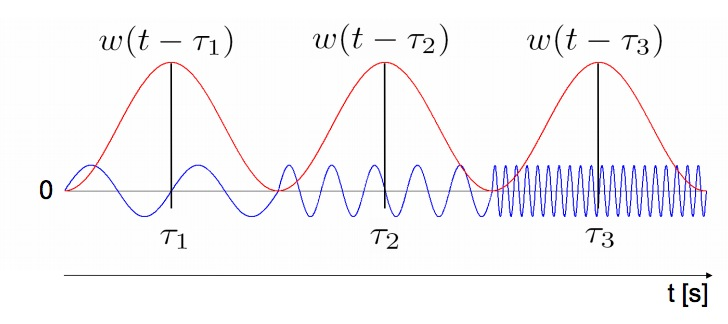
\includegraphics[width=\linewidth]{STFT}
    \end{center}
    \legend{Source: IFN Magdeburg}
    \label{fig:stft}
\end{figure}

The magnitude of the STFT $\vert \bm{X}(\tau,f) \vert $is called spectrogram or power spectrum if the magnitudes have been squared and are often used to provide a graphical display of the spectrogram. Below we will see some examples of powerspectra. Notice the difference between different music styles. Metal and Hip Hop, styles with a big amount of vocals have high magnitudes spread over the whole spectrum and time while more instrumental based styles, like electronic or classical produce more sparse powerspectra with a tendency to higher magnitudes in the lower frequencies. 

\begin{figure}
    \caption{Figure showing logarithmic plots of powerspectra of different musical styles. The spectra were generated using a hamming window function, segment size of 23 milliseconds and an overlap of 50\%.}
    \begin{center}
        
\includegraphics[trim=140 0 140 0, clip, width=\linewidth]{powerspectra}
    \end{center}
    \label{fig:powerspectra}
\end{figure}

\subsection{Acoustical Features}
\subsubsection{Timbral Texture Features}
Many subsequent feature use the magnitude of the power spectrum therefore we introduce $\bm{M}_{t}[n] = \vert \mathbf{X}(\tau,n) \vert^2$. Where $\vert \mathbf{X}(\tau,n) \vert^2$ is the squared magnitude at segment $\tau$ and frequency bin $n$. Subsequently some timbral texture features which are considered relevant by \cite{tzanetakis2002musical} are presented. According to the author these features are standard features proposed for music-speech discrimination and speech-recognition.

\paragraph{Spectral Centroid}
The spectral centroid is a measurement for how bright or how dark a sound sounds. It is therefore a measurement of the spectral shape and is obtained by calculating the centroid of the magnitude spectrum of the STFT of a track.

$$C_{\tau} = \frac{\sum^{N}_{n=1}\bm{M}_{t}[n] * n}{\sum^{N}_{n=1}\bm{M}_{t}[n]}$$

\paragraph{Spectral Rolloff}
The Spectral Rolloff is a feature that measures how much energy resides in the lower frequencies. It is the frequency $R_{t}$ below which some fraction (commonly $0.85$) of the magnitude distribution is concentrated.

$$ \sum_{n=1}^{R_{t}}\bm{M}_{t}[n]  = 0.85 * \sum_{n=1}^{N}\bm{M}_{t}[n] $$

\paragraph{Spectral Flux} This feature is defined as the squared difference between the magnitude of two frames of the powerspectrum. The spectral flux is a measurement of local change in the powerspectrum:

$$ F_{t} = \sum_{n=1}^N (\bm{M}_t[n] - \bm{M}_{t-1}[n])^2$$ 

\paragraph{Time Domain Zero Crossings}
With this feature is the average of how many times the signal crosses the zero amplitude line. It is used as a measurement of noise in the signal. The sign function returns $1$ for positive numbers and $0$ for negative numbers. $x(n)$ is the time-domain signal for segment $\tau$ 

$$Z_\tau = \frac{1}{2}\sum_{n=1}{N}\vert sign(x(n)) - sign(x(n-1))\vert$$

\paragraph{Mel-Frequency Cepstral Coefficients}
MFCC are features that are also based on the STFT. The FFT bins are transformed using triangular filter to fit into Mel Frequency bins. This features have been widely used in speech recognition systems but have also proofed very useful for musical timbre description\cite{logan2000mel}. Later we will present how these features are motivated and calculated in detail.

\subsubsection{Rhythm Features}

\paragraph{Fluctuation Patterns}
Fluctuation Patterns also called Rhythm Patterns are psycho-acoustic, time independent features matrices which describe loudness modulation on various different frequency bands\cite{rauber2002using}. These features have been adjusted to include research about the human perception of audio signals. How these are calculated and how research concerning human perception influences these features will be shown later in this work.

\paragraph{Rhythm Histograms}
Rhythm Histograms are based on Fluctuation Patterns and present a simpler representation of them\cite{lidy2005evaluation}. In contrary to FP these feature do not store rhythmic information on different bands. The modulation magnitudes for all frequencies are summed up to obtain a histogram of rhythmic energy per modulation band. Figure \ref{fig:rhythm_histo} shows the rhythm histograms from the above shown STFT spectra.

\begin{figure}
    \caption{Figure showing 4 example plots of rhythm histograms.}
    \begin{center}
        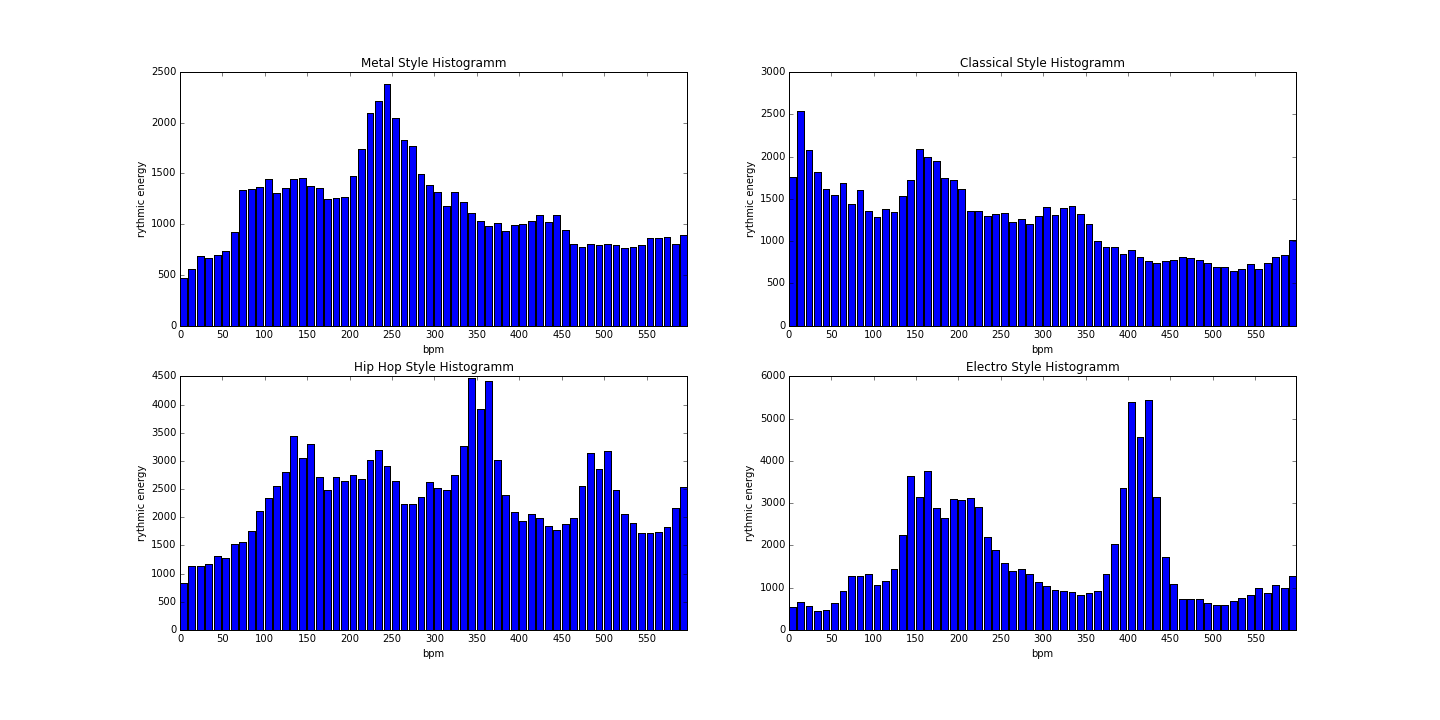
\includegraphics[trim=140 0 140 0, clip, width=\linewidth]{rhythm_hist}
    \end{center}
    \label{fig:rhythm_histo}
\end{figure}

\subsection{Other Features}
It should be mentioned that there exists other techniques besides analysing audio data. Noteworthy is the work \cite{vembu2005self} which tries to make music recommendation by textual mining album reviews. Another interesting approach is to use social tagging websites to retrieve tags for tracks, like done by \cite{hariri2012context}. Using data generated by humans about a musical piece allows to include personal and cultural context into features, which can be very useful as these backgrounds affect how music is perceived as we will see below.

\section{Clustering Techniques}
Ensuing we will present some popular clustering techniques which are similar to the ones we will be using in our approach. Clustering means finding groups of data points in a multidimensional space, whose inter-point distances are small compared with distances to points of other groups\cite{bishop2006pattern}.

\subsection{K-means}
K-means is a well known centroid based clustering technique. To explain this algorithm some notation is introduced. It will be assumed that the number of clusters $K$ is given. For each cluster we define a set of vectors $\bm{\mu}_k$ with $k = 1,\ldots,K$. Let`s assume now that these $\bm{\mu}_k$ represent the centres of our $K$ clusters. The goal is to find an assignment of data points to clusters as well as find the best possible centres for these clusters. To describe the assignment of data points to cluster we introduce for each data point $\mathbf{x}_n$ a set of binary variables $r_{n,k} \in \{0,1\}$, with $k = 1,\ldots,K$. If $x_n$ is assigned to cluster $k$ then $r_{n,k} = 1$ and $r_{n,j} = 0$ for all $j \neq k$. We can than formulate an objective function:

$$J = \sum^{K}_{n=1} \sum^{K}_{k=1} r_{n,k} \norm{\mathbf{x}_n - \bm{\mu}_k}^2$$

These represents the squared distance for each point to it's assigned cluster centre. To minimise the objective function two steps are made. By repeating this two steps convergence to a local minimum is assured\cite{bishop2006pattern}:
\begin{enumerate}
\item Optimise the assignment of the data points to the centres by choosing the nearest center. 
\begin{equation}
r_{n,k} = 
\begin{cases}
1 &\text{if} \text k = \arg \min_j \norm{\mathbf{x}_n - \bm{\mu}_j}^2 \\
0 &\text{otherwise}
\end{cases}
\end{equation}
\item Optimise position of centres. $J$ is a quadratic function of $\mu_k$ to minimise this function we set it's derivative to zero and solve for $\mu_k$ so we obtain:
\begin{equation}
\mu_k = \frac{\sum_n r_{n,k}\mathbf{x}_n}{\sum_n r_{n,k}}
\end{equation}
\end{enumerate}

\subsection{Multivariate Gaussian Mixtures Models}
A mixture of gaussians is a probabilistic model that uses a superposition of $K$ Gaussian densities. This distribution can be used to model almost any continuous density very accurately by using the right amount of components:

\begin{equation} \label{components}
p(\bm{x}) = \sum_{k=1}^K \pi_k \mathcal{N}(\bm{x} \vert \bm{\mu}_k, \bm{\sigma}_k) 
\end{equation}

as can be seen above each component has it's own mean $\bm{\mu}_k$ and it's own covariance $\bm{\sigma}_k$. $\pi_k$ is called the mixing components and governs the form of the distribution. As all probability density function have to be positive we can infer $\pi_k >= 0$ and by integrating \ref{components} we get:
\begin{equation}
\begin{split}
\int p(\bm{x}) d\bm{x} &= \sum_{k=1}^K \pi_k \int \mathcal{N}(\bm{x} \vert \bm{\mu}_k, \bm{\Sigma}_k) d\bm{x} \\
1 &= \sum_{k=1}^K \pi_k
\end{split}
\end{equation}

as the integrals of probability densities are normed to be $1$, we get a further constraint. It holds that $ 0 \leq \pi_k \leq 1$ hence $\pi_k$ can be considered a probability itself and is known as the prior probability of picking the $k^{th}$ component.

Now to find the right parameters of such a mixture distribution to fit the data we can maximise the logarithmic likelihood over all $N$ data points $\bm{X} \in \mathbb{R}^N \times \mathbb{R}^D$ and is given as:

\begin{equation} \label{likelihood}
\ln p(\bm{X} \vert \pi, \mu, \Sigma) = \sum_{n=1}^N ln ( \sum_{k=1}^K \pi_k \mathcal{N}(\bm{x}_n \vert \bm{\mu}_k, \bm{\sigma}_k) )
\end{equation}

This formula is kown to have no closed-form analytical solution \cite{bishop2006pattern} and can therefore only be estimated using an algorithm known as expectation maximisation. In this work we will use a neural network called Incremental Gaussian Mixture Network to estimate the number of components and their respective parameters for each component automatically. It also uses the expectation maximisation algorithm and some heuristics to add or remove components incrementally. For more details and explanations on this algorithm \cite{heinen2010incremental} should be consulted.
To use a Gaussian Mixture Model for clustering it is sufficient to assign each datapoint, after fitting the parameters, to the component corresponding to the highest posterior probability $p(k\vert \bm{x})$ given by the Bayes' theorem:

\begin{equation}
p(k\vert \bm{x}) = \frac{\pi_k \mathcal{N}(\bm{x} \vert \bm{\mu}_k, \bm{\sigma}_k)}{\sum_l \pi_l \mathcal{N}(\bm{x} \vert \bm{\mu}_l, \bm{\sigma}_l)}
\end{equation}


\section{Psychological and Human Aspects}

\subsection{Music Similarity}
As seen above to give recommendation a definition of similarity is inevitable. Many studies have been made concerning music similarity. It was soon noticed that human perception of music similarity does not comply with the definition of an Euclidean metric\cite{berenzweig2004large}. Furthermore music similarity is perceived very subjective by most individuals. Often the perception of similarity is influenced by current mood as well as by the amount of interested someone has in a certain style of music. It is often perceived that people, who aren't interested in a certain style perceive all music as "the same". Moreover music has many distinct dimensionalitys such as tempo, rhythm, tonality, genre, melody, geographical origin, lyric content, and much more \cite{berenzweig2004large}. This permits music similarity to be interpreted on many different dimensions, adding complexity to the problem. Later we will limit these dimension to acoustic similarity.

\subsection{Personality and Cultural Background concerning Musical Perception}
Most of us have experienced how cultural background or personality influence musical taste and perception. For example there has always been a cultural bias against popular music, nowadays lesser than 50 years ago. Some research, concerning preferences in musical styles, published before 1950 contains statements that defines popular music as "music that is ranked by critics as tawdry, banal, insipid"\cite{gernet1940musical}.

Also personality influences preferences in musical styles. In 1939 Burt, published research, which subjected individuals to introvert versus extrovert and stable versus unstable personality tests as devised by Eysenck. He came to the conclusion that stable extroverts prefer solid predictable music in contrast to stable introverts, who enjoy listening to more cognitive classical and baroque styles. It is also interesting that a study conducted in Japan shows that japanese adolescents are more likely to enjoy listening to classical or jazz music than Americans of the same age \cite{wells1998genre}. It was also shown that heavy metal music is generally disliked because of social stigmata associated with it. Another study shows that there are tempo preferences between social groups \cite{uitdenbogerd2002review}. It was also shown that women are more interested in music than men. Moreover it has been shown that people prefer musical styles, which they were listening to during a critical period of their lives, at an average age of about 23.5 years.  

\chapter{The Approach}
In this work it is assumed that acoustic similarity can be used to recommend musical pieces to a user. It is also assumed that the music similarity can be modelled using an euclidean metric for simplicity reasons. The approach presented here makes use of audio features as used in MIR, which have been shown as being good descriptors of musical features. These features are then compressed in their dimensionality and presented to a SOM. After training the network we can assign each track in our database to a cluster. New unknown tracks can also be clustered immediately as the neural network has already been trained using our current database, allowing this recommender system to work online. New tracks can therefore be recommended instantly, without having to wait for sufficient user data about them being available. This clustering is then used as a similarity measure between tracks. We then examine a users previous likes and their relative distribution among these clusters to give recommendation on similar tracks.

\section{Data Acquisition}
It proofed quite difficult to obtain a dataset for this approach. Most datasets provided for music information retrieval are very small and provide no user data at all. Furthermore they are often limit to unrealistic genres. We will describe how a realistic dataset was constructed to provide audio as well as user preference data.


\subsection{Data Sources}
To obtain audio data as well as user data for evaluation, a subset of the Million Song Database \cite{Bertin-Mahieux2011} was used, as it provides sufficient metadata as well as track ids from services like 7digital to obtain preview audio. Furthermore we used the ThisIsMyJam archive dump\cite{janssonmy} to get user data on tracks. ThisIsMyJam was a social music website where users could post their current favourite track from various sources. It was possible to follow other users as well as to like other users jams. We preferred this dataset over the TasteProfile dataset as it contains explicit likes from users in contrary to listening history, which also presents preferences but in a implicit form.

\subsection{Constructing the subset}
As Audio as well as user data is needed we constructed a subset of the MSD to include all these requisites. This subset was constructed as follows:

\begin{enumerate}

\item The ThisIsMyJam dump likes file was constrained to obtain a list of likes which refer to songs known to the MSD. To achieve this we used a mapping from jam ids to MSD ids provided by the LabROSE.

\item To limit computational costs we randomly sampled 250 users from this data. This 250 users made 14489 likes which matched to 8496 distinct MSD tracks.

\item  To get audio data for each track the 7digital API was queried by preferring track ids obtained from the MSD if available. If not available album id, artists ids or text search where used to find the correct audio file. 7digital provides preview audio files with a length of 30 to 60 seconds. After querying it was possible to obtain 8003 audio files.

\item we restrict our subset of likes and tracks to the tracks, for which audio previews could be obtained.

\end{enumerate}

Finally the subset consists of $250$ distinct users with $13891$ likes and $8003$ distinct tracks with audio files.

\subsection{Genre Distribution}
For about 6000 tracks genre attributes could be obtained using the tagtraum genre annotations \cite{schreiber2015improving} as well as the MAGD dataset. In Figure \ref{fig:genres} we can see that the data is very unbalanced and almost $50\%$ are Pop/Rock songs.

\begin{figure}
    \caption{Genre annotations for 6000 tracks of the constructed subset}
    \begin{center}
        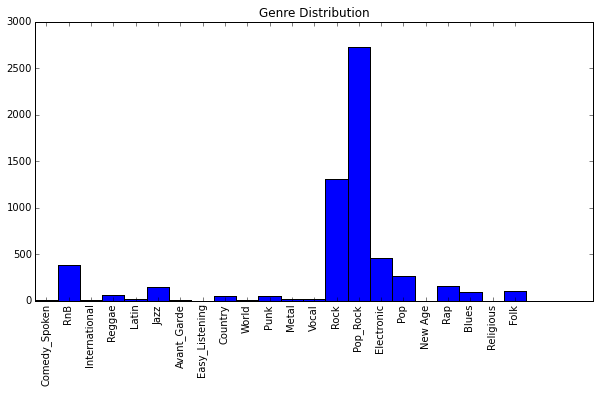
\includegraphics[width=\linewidth]{genres}
    \end{center}
    \label{fig:genres}
\end{figure}

\section{Audio Features}
The features chosen to form feature vectors for our recommender system are Fluctuation Patterns and Mel-Frequency Cepstral Coefficients as they are popular in other research fields and have been proven to provide good results for most musical domains.
%TODO citation

\subsection{Preprocessing Audio} \label{sec:preprocessing}
To reduce computational complexity some preprocessing is done to reduce the input data. First the raw audio data is combined into one mono channel. Then the audio is sampled down to $11025Hz$. Next the data is segmented into 6s chunks and intro and outro chunks are removed. If the audio track is longer than $30 seconds$ every third chunk is removed.

\subsection{Mel-Frequency Cepstral Coefficients}
MFCC is short for Mel-Frequency Cepstral Coefficients. These are short-term spectral based features. This means they usually are time dependent and offer therefore a description of timbre evolution over time. Although MFCCs were designed for speech recognition they also proofed to be very useful in music analysis \cite{logan2000mel}. The Computation of MFCCs is oriented at the model of speech production, which claims that speech is modelled by a linear system. The excitation signal generated by the vocal cords is thereby enveloped by the impulse response of the vocal tract \cite{niemann2013klassifikation}. For speech-recognition the excitation signal is irrelevant, important is only the slow change of the vocal tract, which determines the spoken sound. The folding is converted into an addition by taking the cepstrum and can therefore be separated more easily from the excitation.

\begin{enumerate}

\item \textbf{Calculating the Powerspectrum} \\ The powerspectrum of the preprocessed audio is computed by squaring the spectrum obtained from STFT as described in \ref{section:STFT}, using a segment size of 256 samples which corresponds to 23ms and a Hanning window with 50\% overlap, yielding the matrix $\bm{X}$.

\item \textbf{Taking the logarithm} \\ Little is found about the motivation of this step in literature. Most probably it accounts for the phenomena that loudness is not perceived linear.

$$\bm{X}'(i,j) = \log (\bm{X}(i,j))$$

\item \textbf{Map to Mel Scale} \\ The coefficient of the logarithmic power spectrum $X'$ are summated into mel bin using triangular filter banks. The correlation between frequency and perceived pitch is none linear and can be expressed by:

$$f_{mel}(f_{Hz}) = 1125 * \log(1+\frac{f_{Hz}}{700})$$

To obtain the triangular filter bank a linear spacing defining the desired number of mel bins $N=40$ is done in the mel domain resulting in a vector $\bm{l}_{mel}$ containing upper and lower limits of the bins. This vector is then transformed back into frequency domain using the inverse of the above function $f_{mel}$. To compute the right indexes a helper function $binfreq: [1,\ldots, 256] \rightarrow \mathbb{R}$ has to be introduced. This function shall return the associated frequency considered with the bin index.

\begin{equation}
\begin{split}
\bm{l}_{Hz}(i) &= f_{mel}^{-1}(\bm{l}_{mel}(i)) \\
idx_i &= \{ j \vert binfreq(j) \geq \bm{l}_{Hz}(i) \land binfreq(j) < \bm{l}_{Hz}(i+1) \} \\
\bm{C}_{mel}(i,j) &= \sum_{k \in idx_i} \bm{X}'(k,j)
\end{split}
\end{equation}

\item \textbf{Apply the DCT} \\ The frames in $\bm{C}_{mel}$ are usually highly correlated. To reduce the number of parameters usually a Discrete Cosine Transform (DCT) is applied to each frame to decorrelate the components. Theoretically the DCT is an approximation to the Principal Component Analysis and is used as it is fast and domain independent. Only the first 13 cepstral feature are kept from each vector.

\end{enumerate}

\subsection{Fluctuation Patterns}
As mentioned above Fluctuation Patterns provide a time independent feature for music rhythm description, while considering characteristics of human auditorial perception. It follows a description of multiple steps on how to compute these features and how these steps are motivated. The process of computing fluctuation patterns can be split into two major parts: Calculating the Specific Loudness Sensation and computing the Rhythm Patterns, as proposed by \cite{pampalk2001islands}.
\subsubsection{Specific Loudness Sensation}
In this step some psychoacoustics scales and filter are applied to the STFT of the preprocessed audio data. This involves 6 steps:
\begin{enumerate}

\item \textbf{Calculating the Powerspectrum} \\ The powerspectrum of the preprocessed audio is computed by squaring the spectrum obtained from STFT as described in \ref{section:STFT}, using a segment size of 256 samples which corresponds to 23ms and a Hanning window with 50\% overlap.

\item \textbf{Bark Critical Bands} \\ According to \cite{fastl2007psychoacoustics} our inner ear separates certain frequencies and concentrates them on certain parts of our basilar membrane. So the inner ear can be regarded as a set of asymmetrical bandpass filters. These bandpass filters have centre frequencies related to the ones of the bark scale. The position and width of these bands has been analysed in psycho-acoustical experiments by using a loud tone to mask a quiet one. At high frequencies the frequency difference of these two tones must be greater so that listeners can hear the quiet tone, at lower frequencies the quiet tone can be perceived at smaller differences. Moreover these masking effects are closely related to noticeable frequency variations. Therefore two tones within a critical band are very hard to distinguish. Listeners usually can't tell which one of the two is higher or lower. %describe how bandpass filters are applied to spectrum

\begin{figure}
    \caption{Bark scale}
    \begin{center}
        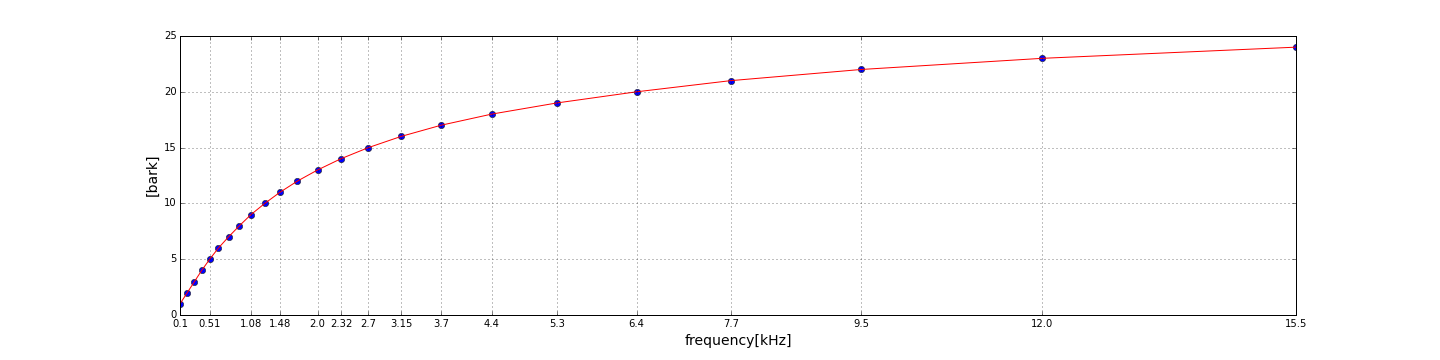
\includegraphics[width=\linewidth]{bark}
    \end{center}
    \label{fig:bark}
\end{figure}

\item \textbf{Spectral Masking} \\ As mentioned above a louder tone can mask a quieter one, if they are played simultaneously or shortly before or after. This can also occur across critical bands and is a natural phenomena that helps to reduce noise. A spreading function has been proposed to account for the effects of simultaneous masking\cite{schroeder1979optimizing, pampalk2001islands}. The spreading function is applied to each frame of our critical band rate spectrum matrix and describes the influence of the $i^{th}$ band on the $j^{th}$, visualised in Figure \ref{fig:spreading_func}: 

$$\mathbf{S}(i,j) = 15.81 + 7.5(i-j + 0.474) - 17.5 \sqrt{1+(i-j+0.474)^2}$$

To apply the spreading function to each frame of our matrix we can simply multiply the spreading matrix with the critical band rate spectrum matrix $\mathbf{B}$:
\begin{equation}
\begin{split}
\mathbf{B}_s(i,t) &= \sum_{j=1}^{24} \mathbf{S}(i,j) \mathbf{B}(j,t), \text{this is equivalent to} \\
\mathbf{B}_s &= \mathbf{S} \mathbf{B}
\end{split}
\end{equation}

In Figure \ref{fig:sm_ex} is demonstrated how spectral masking affects the critical bands. Higher frequencies are affected more than lower ones, these can be observed especial in the profile plot. The two right plots of the vertical matrix demonstrate that it only affects single frames. 


\begin{figure}
    \caption{Logarithmic plot of $S$, notice the asymmetrical shape}
    \begin{center}
        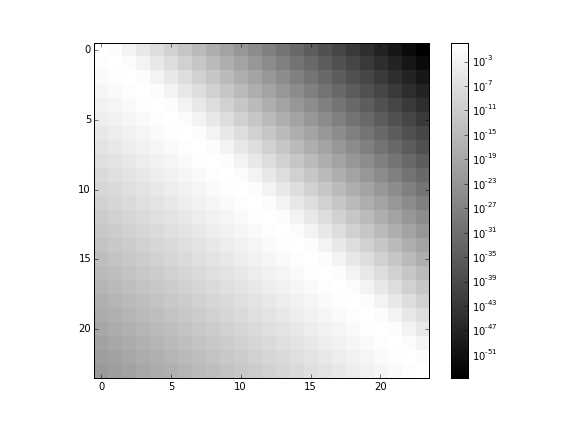
\includegraphics[width=\linewidth]{masking}
    \end{center}
    \label{fig:spreading_func}
\end{figure}

\begin{figure}
    \caption{Examples of how spreading affects the critical bands}
    \begin{center}
        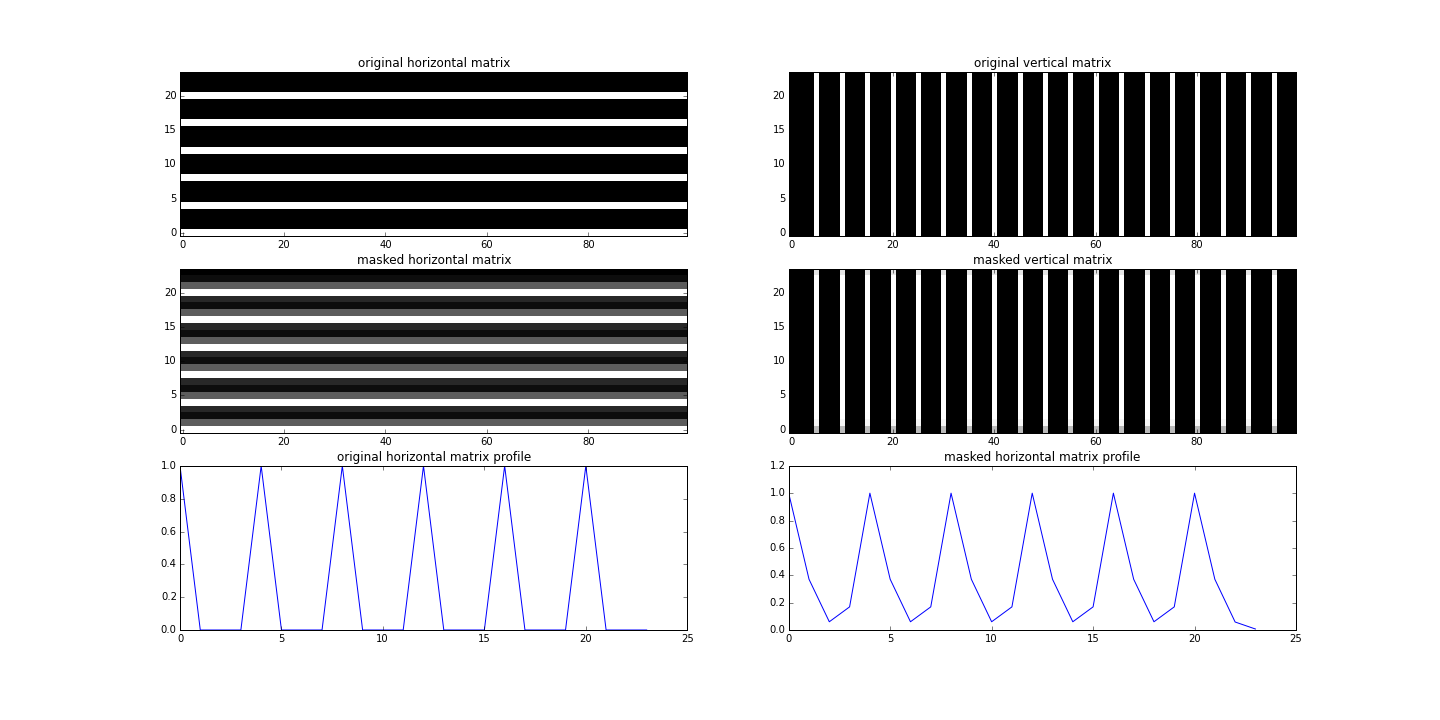
\includegraphics[trim=140 0 140 0, clip, width=\linewidth]{masking_examples}
    \end{center}
    \label{fig:sm_ex}
\end{figure}

\item \textbf{Decibel Scale} \\ To proceed the values of our matrix $B_S$ have to be converted into the decibel scale. The decibel is a logarithmic scale which measures the ratio between two numbers. As the human hearing is possible to perceive a rather large range from the lowest to the loudest sound in terms of sound pressure level, approximately $10^{12}:1$. The decibel scale offers a much more convenient way to represent these numbers, by mapping those to a more manageable range between $1$ and $140$. As the decibel scale is a relative scale it uses instead of a zero point, a reference point, which can be arbitrary. Sound amplitudes are most often measured using sound pressure levels (SPL) as are our digital audio archives based on SPL, which measures amplitudes in terms of $dynes/cm^2$ or Pascal. Usually the reference point used for this unit is $20\mu Pa$ as these represents the hearing threshold of a sound at $1000kHz$ \cite{lass2012review}, which as already mentioned is quite popular in acoustics. To calculate decibels based on sound pressure levels from audio archives some adjustments have to be made. As our data is represented in bits we will define the lowest possible sound as $1$ (or $-1$, as we use magnitudes). The conversion from SPL to decibel is given by:

$$ dB (SPL) = 20 * \log(\frac{p}{p_0}) $$

Whereas $p_0$ is the hearing threshold defined as $1$. By applying this formula to each entry of our matrix $\mathbf{B}_S$ a loudness matrix is obtained. It is necessary to define all entries lower than one to one $\mathbf{B}_S'$ to avoid the singularity of the $\log$ function.
\begin{equation}
\begin{split}
\mathbf{B}_S'(i,j) &= 
\begin{cases}
1, &\quad \text{if} \quad \mathbf{B}_S(i,j) < 1 \\ 
\mathbf{B}_S(i,j) &\quad \text{otherwise}
\end{cases}\\
\mathbf{L}_{dB}(i,j) &= 20 * \log_{10}(\mathbf{B}_S'(i,j))
\end{split}
\end{equation}

\item \textbf{Phon Scale} \\ How we perceive loudness at different frequencies is not linear. To account for this effect the phone scale is introduced which allows to map our matrix's values to phon. The phon makes loudness sensation independent from the frequency. A tone at any frequency with 40 phon is defined to be as loud as a 40dB tone at 1kHz. The equal loudness contours in \ref{fig:phon} have been obtained by experiments involving single tones. These contours achieve a minimum around 2kHz to 5kHz which are the frequencies humans are most sensible to. Outside these interval the curves rise rapidly corresponding to decrease in hearing sensibility outside this interval. To obtain the phon representation $\mathbf{L}_{phon}$ of the loudness matrix $\mathbf{L}_{dB}$, we define the equal loudness contour matrix $\mathbf{C}_{elc}(i,j)$ which contains the in Figure \ref{fig:phon} plotted curves, with the decibel value of $j^{th}$ contour at the $i^{th}$ critical band (represented as black dots in Figure \ref{fig:phon}). The corresponding phon values can then be interpolated, using $\mathbf{c}_{phon} = [3,20,40,60,80,100]$ as follows:

\begin{enumerate}
\item Cast values below contour of phon 3 to smallest available dB value.
\begin{align*}
\mathbf{L}_{db}'(i,t) &= max(\mathbf{L}_{db}(i,t), \mathbf{C}_{elc}(i,1))
\intertext{\item for each entry find upper contour index}
level_{i,t} &= \arg \min_{j} ( \mathbf{L}_{db}'(i,t) <  \mathbf{C}_{elc}(i,j))
\intertext{\item Linear interpolation first step: $r_{i,t}$ being the relative distance to the lower level}
r_{i,t} &= \frac{ \mathbf{L}_{db}'(i,t) - \mathbf{C}_{elc}(i,level_{i,t}-1)} {\mathbf{C}_{elc}(i,level_{i,t}) - \mathbf{C}_{elc}(i,levels_{i,t}-1) } 
\intertext{\item Linear Interpolation second step: compute interpolated value}
\mathbf{L}_{phon}(i,t) &= \mathbf{c}_{phon}(level_{i,t} -1) +r_{i,t} \mathbf{c}_{phon}(level_{i,t} ) 
\end{align*}
\end{enumerate}



\begin{figure}
    \caption{The phone contours}
    \begin{center}
        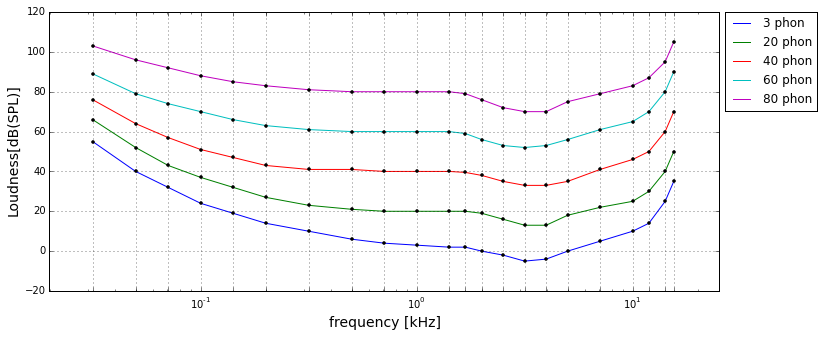
\includegraphics[width=\linewidth]{phon}
    \end{center}
    \label{fig:phon}
\end{figure}

\item \textbf{Sone Scale} \\ Notice that phon scale is not linear as doubling the phon does not result in a doubled loudness perception. To transform the phon unit into a linear scale the sone scale is used, which represents perceived loudness in a linear scale. How the phone scale relates to the sone scale can be seen in figure \ref{fig:sone}. The conversion is calculated as follows:
\begin{equation}
\bm{L}_{sone}(i,t) = 
\begin{cases}
2^{\frac{1}{10}(\bm{L}_{phon}(i,t)-40)} &\quad \text{if} \quad \bm{L}_{phon}(i,j) > 40\\
(\frac{1}{40}\bm{L}_{phon}(i,t))^{2.642} &\quad \text{otherwise}
\end{cases}
\end{equation}

\begin{figure}
    \caption{Relation between loudness sensation and loudness level}
    \begin{center}
        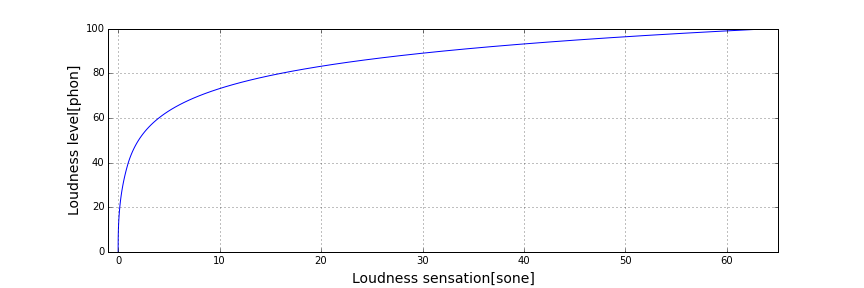
\includegraphics[width=\linewidth]{sone}
    \end{center}
    \label{fig:sone}
\end{figure}

\end{enumerate}

\subsubsection{Rhythm Patterns}
Until now the obtained feature matrix from last section $\bm{L}_{sone}$ is still time dependent. Shifts in the signal of the same music would result in highly dissimilar matrices, making this feature vector unsuitable for classification. Hence Rhythm Patterns are introduced to obtain a time invariant representation of the loudness sensation.

If we examine the loudness of a specific band we will observe that it rises and falls several times. This is likely to occur in a periodical pattern, which is perceived as the rhythm. Usually instruments follow a rhythmic pattern which is very accurately timed this as perceivable in the critical bands. This can be seen in Figure \ref{fig:periodicity}, a plot of several critical bands using $\bm{L}_{sone}$ of an electronic music track. As we can see there is some periodicity especially in the lower bands as electronic music uses mostly simple rhythms at low frequencies (commonly mown as beats). It is also noteworthy to examine all these critical bands overlaid in a single plot, as peaks repeatedly meet at a certain periodicity, which can be interpreted as a musical bar, a time segmentation most musicians use to time their compositions. If we consider this periodical pattern as a linear combination of sinuids in a discrete sampled domain we can use the FFT to reconstruct the amplitude corresponding to each frequency for each individual critical band. A 3-step approach, proposed by \cite{rauber2002using}, is presented subsequently to construct time independent rhythm descriptors with psycho-acoustic considerations.

\begin{figure}
    \caption{Loudness modulation in certain critical bands of an electronic music piece. Observe the periodicity especially in lower bands and in the last plot.}
    \begin{center}
        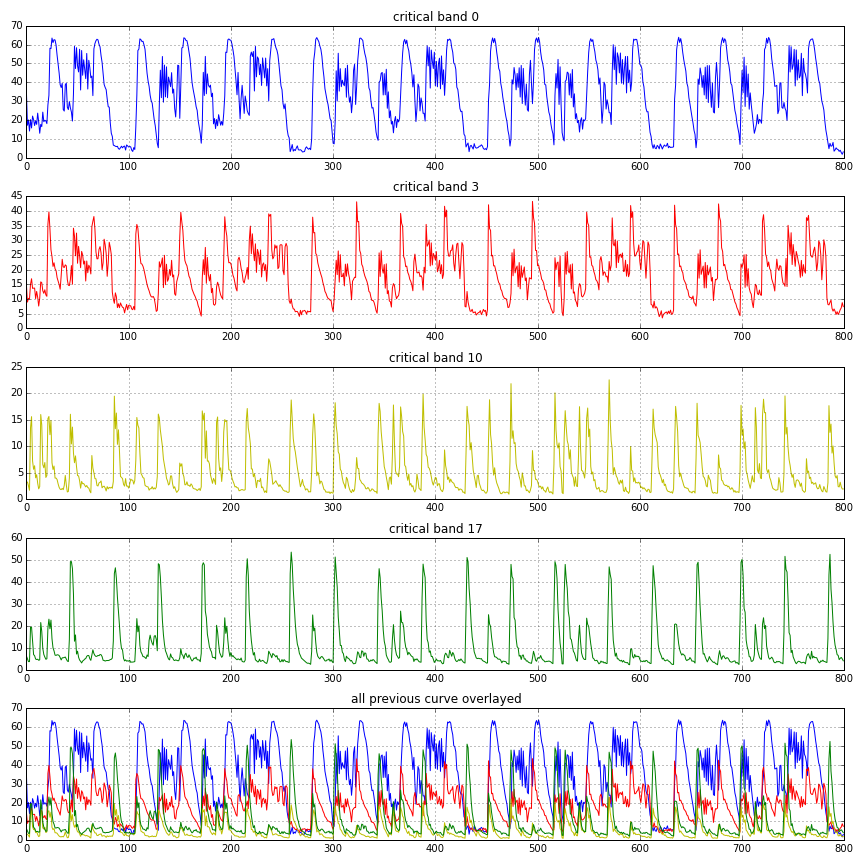
\includegraphics[width=\linewidth]{periodicity}
    \end{center}
    \label{fig:periodicity}
\end{figure}

\begin{enumerate}
\item \textbf{Amplitude Modulated Loudness} \\ As described above each critical band is likely to have some periodic phenomena. Consequently we will analyse the underlying modulation frequencies. These analysis is done for each 6 second segment, described in \ref{sec:preprocessing}. As a result of the STFT we have time quanta of $12ms$. Applying a FFT on each of this 6 second segments will result in a spectrum with frequency bin from $0Hz$ to $43Hz$ with an accuracy of $0.17Hz$. Note that a modulation frequency of $43Hz$ corresponds to approximately $2600$ beats per minute (bpm). The modulation amplitude is calculated as follows:

$$\bm{\Delta L}_s(i) = FFT(\bm{L}_{sone}(i,s*[1, \ldots, 512]))$$

With $\bm{L}_{sone}(i,s*[1, \ldots, 512])$ being the $i^{th}$ critical band of $s^{th}$ $6s$ segment.

\item \textbf{Fluctuation Strength} \\ the hearing sensation produced by slow amplitude fluctuation, usually less then $20/s$,  is called fluctuation strength. Sensation induced by faster fluctuations are called roughness \cite{fastl1982fluctuation}. It was discovered that fluctuation strength is most intense around modulation frequencies of $4Hz$ an gradually decreases until reaching $15Hz$. After $15Hz$ the sensation of roughness starts to increase. It was shown that the absence of roughness is a prerequisite for musical consonance \cite{fastl1982fluctuation}. To take the unequal sensation of fluctuation strength into account a weighting function $f:\mathbb{R} \rightarrow [0;1]$ based on Fastl's model is introduced an shown in Figure \ref{fig:fs_model}. With this function fluctuation modulations around $4Hz$ are emphasised. 

$$\bm{F}_s(i,j) = \bm{\Delta L}_s(i,j) * f(j)$$

As after $15Hz$ roughness starts to increase a summary of all track's fluctuation strengths are plotted in Figure\ref{fig:summary}. It can be observed that after $10Hz$ there is hardly any activity. Consequently only the first $60$ values which correspond to $10Hz$ are used.

\begin{figure}
    \caption{fluctuation strength model}
    \begin{center}
        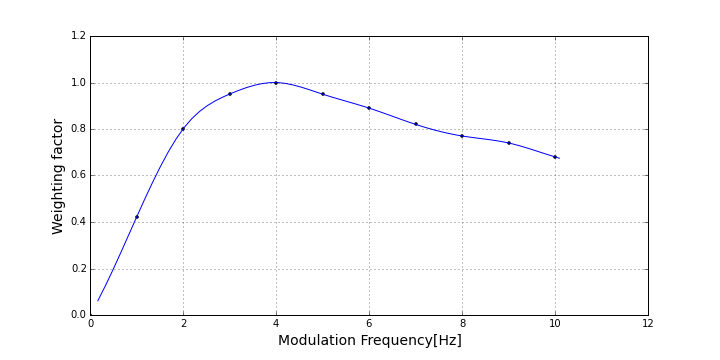
\includegraphics[width=\linewidth]{fs_model}
    \end{center}
    \label{fig:fs_model}
\end{figure}

\item \textbf{Modified Fluctuation Strength} \\ At this point we have time independent rhythm descriptors which would already provide good results. To further improve this features \cite{rauber2002using} applies gradient filter to enhance vertical lines in the matrices which occur in beat rich music styles. Afterwards a gaussian filter is applied to blur across critical bands as the exact bands are irrelevant for music similarity. This measures reduce the Euclidean distance between two similar music pieces, which is a desired effect. 
\end{enumerate}

\subsubsection{Examples of Modified Fluctuation Patterns}
In this section we will present some examples of fluctuation patterns and discuss their similarities and distances in music space. Figure \ref{fig:fp_examples} shows 4 fluctuation pattern matrices of 4 different tracks each of a distinct musical style and Table \ref{tab:distances} shows the distances between normalized and compressed fluctuation patterns. Observe how Hip Hop and Electro tracks produce kind of similar fluctuation  patterns as they both have a very bass and beat based rhythms. They still are distinct as the Hip Hop track has a lot of fluctuation also in higher bands but they are compared to the beat loudness rather small and spread over all frequencies therefor less visible in the plot. The Electro track has only a smaller peak at around $400bpm$ in higher frequencies, which are percussive instruments like hi-hats. Therefore they are still distinct enough as can be seen in distance matrix they have the biggest distance between all pairs. It might seem surprisingly that metal and classic music have the lowest distance between each other, but observing the fluctuation patterns we can see that they are quite similar in rhythmic composition. Beethoven's Piano Sonata is a quite lively piano pieces with many different notes played in fast sequences with varying loudnesses. This can be interpreted as similar to a Metal track which usually has a lot of guitar chords played in fast sequence just shifted a little into upper frequencies. Still there are quite some differences for example the classic tracks has many peaks whereas the metal track as a single beat around $250bpm$ which is most probably the bass drum. Also the scales are very different the metal track is way louder as can be seen on the values on it's colour scale.


\begin{figure}
    \caption{Examples of Fluctuation Patterns}
    \begin{center}
        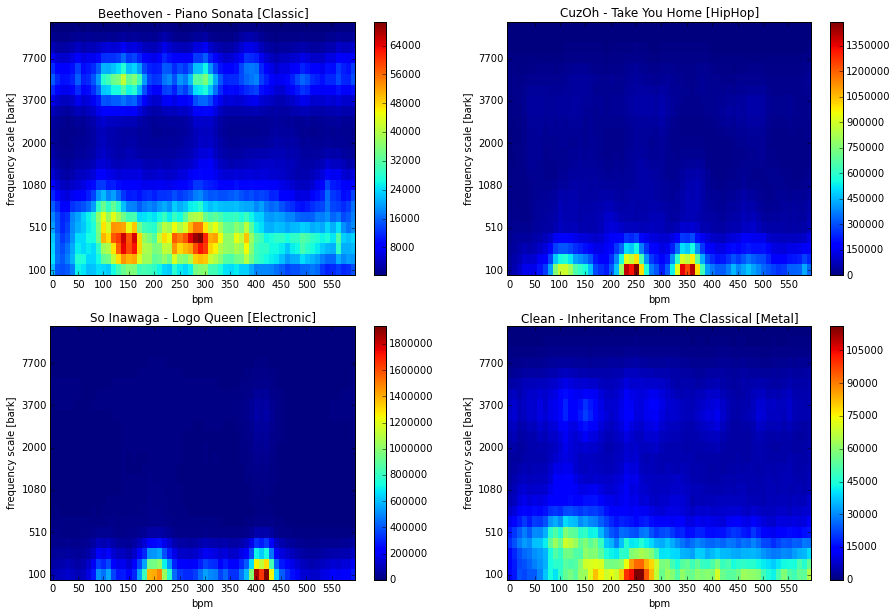
\includegraphics[width=\linewidth]{fp_examples}
    \end{center}
    \label{fig:fp_examples}
\end{figure}


\begin{table}
\center
\caption{Distance matrix between sample tracks}
\begin{tabular}{ r | c  c  c  c  }

& \rot{Classic} & \rot{Electronic} & \rot{Metal} & \rot{HipHop} \\ 
Classic & 0.000 & 5.824 & 1.694 & 4.584 \\ 
Electronic & 5.824 & 0.000 & 5.782 & 6.215 \\ 
Metal & 1.694 & 5.782 & 0.000 & 4.608 \\ 
HipHop & 4.584 & 6.215 & 4.608 & 0.000 \\ 

\end{tabular}
\label{tab:distances}
\end{table}


\section{Feature Combination}
Now there exists a Fluctuation Pattern matrix for every 6s chunk of every track in the database and a for every 6 second chunk exists a matrix with MFCC containing a timbre vector for every $23ms$. As these data amounts are still to big to handle for most clustering algorithms the data has to reduced. The question arrises from the 6s chunks which one represents best the songs rhythm and how can we express the songs timbre dynamically without needing big amounts of data. In the following section we will present various approaches to achieve this. In the Evaluation chapter we will see how these different strategies preform.
 

\subsection{Fluctuation Pattern Dimensionality Reduction}
The Fluctuation pattern matrix has dimenionality of 1440 as we have 24 frequencies in the first dimension and 60 modulation frequencies in the second dimension. As this is to big to achieve a stable clustering, the data is reduced using PCA to a dimensionality of 60. 

\subsubsection{Chunk Selection}
As shown by \cite{pampalk2001islands} the simplest and quite good preforming method to compress all chunks is to calculate the median between all $6s$ chunks. Leaving a single fluctuation pattern matrix to be further compressed using PCA.

\subsubsection{Principal Component Analysis} \label{section:pca}
The principal component Analysis or PCA is a method used here for dimensionality reduction. The PCA is a projection of data of dimensionality $D$ into a subspace of dimensionality $M$ while minimising the average projection cost, which is defined as the squared distance between data points and their projections. To calculate the we have to select a basis of vectors so that the cost function is minimised. To do this let's assume we have complete orthonormal basis of $D$-dimensional vectors $\bm{u}_i$. Then each data point $\bm{x}_n$ can be represented as:

\begin{equation}
\bm{x}_n = \sum_{i = 1}^{D} (\bm{x}_n^T \bm{u}_i) \bm{u}_i
\end{equation}

To achieve dimensionality reduction we have to restrict the number of basis vectors to be $M$. Therefore we can write the projected points $\bm{\tilde{x}}_n$ as:

\begin{equation}
\bm{\tilde{x}}_n = \sum_{i = 1}^{M} z_{ni} \bm{u}_i + \sum_{i = M+1}^{D} b_{i} \bm{u}_i 
\end{equation}

Here $z_{ni}$ depends on each datapoint and basis vector and $b_{i}$ are constants. Our projection cost function is defined as:
 
\begin{equation}
J = \sum_{i = 1}^{N} \norm{\bm{x}_n - \bm{\tilde{x}}_n}
\end{equation}

By setting the derivatives of $J$ to zero and substituting $z_{ni}$ and $b_i$ we get an expression of the distortion measure dependent only on $\bm{u}_i$ \cite{bishop2006pattern}

\begin{equation} \label{cost_func}
J = \sum_{i = M+1}^{D} \bm{u}_i^T \bm{S} \bm{u}_i 
\end{equation}

To minimize this term we have to avoid the trivial result $\bm{u}_i = 0$, to do this we introduce the constraint $\bm{u}_i^T\bm{u}_i = 1$ leading to an modified cost function:

\begin{equation}
\tilde{J} = \sum_{i = M+1}^{D} \bm{u}_i^T \bm{S} \bm{u}_i  + \lambda_i (1-\bm{u}_i^T\bm{u}_i )
\end{equation}

By setting the derivative to zero we can see that this terms reduces to choosing $\bm{u}_i$ to be an eigenvectors of the covariance matrix.

\begin{equation}
\bm{S}\bm{u}_i = \lambda_i \bm{u}_i
\end{equation}

using this observation and substituting this into \ref{cost_func} get our final projection costs function:

\begin{equation}
\tilde{J} = \sum_{i = M+1}^{D} \lambda_i
\end{equation}

We can minimise this function by choosing the residual vectors $\bm{u}_i$, with $i = M+1, \ldots, D$, to be the vectors with the corresponding smallest eigenvalues. Therefore we have to choose as basis vectors the vectors with the biggest eigenvalues in $\bm{S}$. This can be done with a singular value decomposition, which returns a matrix with eigenvalues on the diagonal sorted by size. To project a given vector $\bm{x}_n$ it is sufficient to multiply it with a matrix that has the $M$ used eigenvectors of $S$ in it's rows.

\subsubsection{Quality of PCA}
show reconstruction of fluctuation patterns using principal components

\subsection{Expressing Music Timbre with MFCCs}
Music timbre, also known as tone colour or tone quality in psychoacoustics, is what makes the same tones played with same loudness on distinct instruments sound different. In the following three different approaches to capture dynamic evolution in music timbre are presented. Combining these approaches will lead to 4 distinct feature vectors for music timbre representation.

\subsubsection{MFCC Deltas}
Calculating the delta-cepstrals of MFCCs has been proposed in the automatic speech recognition research community by \cite{furui1986speaker}. In hope to add dynamic information to the static MFCCs. These makes sense also for music as music evolves over time and these dynamics influence the timbre perceived by humans. It was shown by \cite{kumar2011delta} that adding this dynamic component as a feature enhances the speech recognition systems it was also shown that double-delta feature further improve the system but in this work only single delta features are used. To calculate the delta features the following formula was used:

$$\bm{D}_{mel}[n] = \bm{C}_{mel}[n+m] - \bm{C}_{mel}[n-m]$$

Where $ \bm{C}_{mel}[n]$ is a single row vector at position $n$ of the MFCC matrix. The variable $m$ is usually in practive between $2$ or $3$.

\subsubsection{Concatenated MFCCs}
Another idea to represent dynamics is to concatenate multiple MFCC vectors into one vector. Describing a short changes of timbre for a musical piece. This has been done with ten such vectors leading to a feature vector of size $130$. Consequently representing timbre evolution over a timeframe of $230ms$. As the double-deltas have shown to provide further improvement the same was done for the above calculated MFCC deltas. As a feature vector of $130$ is still big another two more PCA over all concatenated MFCCs and Delta MFFCs were executed and the data was compressed to a dimenionality of $40$.

\subsubsection{Medians}
As medians have proofed successful with Fluctuation Patterns and provide a simple and cost effective way of compressing the various vector into a single one, the medians of MFCCs as well as Deltas are computed and stored for feature combinations.

\subsubsection{Polyphonic Timbre} 
It has been shown that MFCCs can be described very good with GMMs. But the methods used to compare GMMs are rather numerical unstable. To overcome this problem a polyphonic timbre representation for MFCCs was used as proposed by \cite{yoshii2008efficient}. These features were used in a hybrid recommender system approach and delivered very good results on japanese music hits. This methods describes a songs timbre as a vector of weights for each gaussian component in a track. To calculate the polyphonic representation of timbre a IGMN \cite{heinen2010incremental} instance was trained over all concatenated MFCCs of all songs resulting in 30 components. These proofed to be quite difficult due to numerical problems caused by the dimensionality of the data. Therefore the compressed version of the concatenated MFFC version was used. Each song is then represented as $30$ dimensional feature vector $\bm{u}$ describing the sum of the probabilities for each vector belonging to each component:

$$\bm{u}(i) = \frac{1}{\vert M \vert} \sum_{m \in M} P(i\vert x_m), \quad \text{for } i = 1, \ldots, 30 $$

With $m$ being the single feature vectors of one song and $P(i\vert x_m)$ being the posterior probability of $x_m$ belonging to the $i^{th}$ gaussian component. 


\subsection{Building Feature Vectors}
From the above calculated features some combinations between them are combined to form the final track representations. The table \ref{tab:feature_vec} illustrates how the vectors are combined, their resulting dimensionality as well as an abbreviation for them to be used subsequently.

\begin{table}
\center
\caption{Feature Vectors}
\resizebox{\linewidth}{!}{
\begin{tabular}{| l | l | c | }
 \hline 
\rowcolor{lightgray} Abb. & Combination & Dimensionality \\ \hline 
\bf{A} & Fluctuation Patterns Compressed + Gaussian Representation of Concatenated MFCC  & $90$ \\ \hline
\bf{B} & Fluctuation Patterns Compressed + Concatenated MFCC Median  & $100$ \\ \hline
\bf{C} & Fluctuation Patterns Compressed + Concatenated MFCC Delta Median  & $100$ \\ \hline
\bf{D} & Fluctuation Patterns Compressed +(Concatenated MFCC + Concatenated MFCC Delta) Median  & $140$ \\ \hline
\bf{E} & Fluctuation Patterns Compressed  & $60$ \\ \hline
\bf{F} & Concatenated MFCC  Medians & $40$ \\ \hline
\bf{G} & Concatenated MFCC Delta Median  & $40$ \\ \hline
\bf{H} & Concatenated MFCC + Concatenated MFCC Delta Median  & $80$ \\ \hline
\bf{I} & Gaussian Representation of Concatenated MFCC  & $30$ \\ \hline
\bf{J} & Fluctuation Patterns Raw  & $1440$ \\ \hline
\end{tabular}}
\label{tab:feature_vec}
\end{table}



\section{Clustering}
Given the above feature vectors it is necessary to order them into distinct clusters. This should be done considering auditory similarity of the tracks. To perform clustering the SOM algorithm was chosen as it is a sophisticated algorithm which can perform unsupervised learning and offers good ways to visualise high dimensional data. This is important as our data contains no explicit information about similarity. Thus the algorithm used must learn by itself which tracks are similar and which are not. After training the SOM we perform a KMeans clustering on the trained codebook to further reduce the amount of clusters. We use the SOMpy implementation by \cite{sompy}, which proofed extremely fast an useful in visualisation tasks.

\subsection{Self-organising Map Algorithm}
The Self-organising Map as introduced by \cite{kohonen2012self} is neural network model inspired by certain regions of the brain which underly a 2 dimensional organization. It usually employs a two-dimensional grid of neural cells or neurons, which are all interconnected with each other. This neurons are identified by their position in two-dimensional space $\bm{r} \in A \subset \mathbb{R}^2$. Each cell is provided with the actual input $\bm{v} \in \mathbb{R}^d$ and has an weight vector $\bm{w_r} \in \mathbb{R}^d$, describing the synaptic strengths for each input element from $\bm{v}$, associated to it. A single iteration of the algorithm, in which all available data vectors $\bm{v}$ are presented to the net is described in the following steps:

\begin{enumerate}
\item \textbf{Initialization} \\ To initialise the SOM appropriate values for all $\bm{w_r}$ have to be chosen. This can be random values if priori information about the data is available. In this approach the principal components (see \ref{section:pca}) of the data are used to initialise the weight vectors which leads to a faster convergence and therefore to lesser iterations.

\item \textbf{Choice of Input} \\ A random data vector $\bm{v}$ is chosen from all available vectors to be presented to the network.

\item \textbf{Excitation Response} \\ The most excited neuron is called the best matching unit or the excitation centre. To calculate a neurone excitation the euclidean distance to its weight vector is used. Te neuron with the weight vector of the smallest distance to the current input $\bm{v}$ is selected as follows:

$$ \norm{\bm{v} - \bm{w_{r'}}} \leq \norm{\bm{v} - \bm{w_r}} \quad \text{,for all} \quad \bm{r} \in A $$

\item \textbf{Adaptation Step} \\ This learning step is carried out by updating all neurons weight's based on a centroid calculation between old and new synaptic strengths as shown below:

$$\bm{w_r}^{new} = \bm{w_r}^{old} + \eta(t) h_{\bm{rr'}}(t)(\bm{v} - \bm{w_r}^{old})$$

and continue at step 2.

\end{enumerate}
With $\eta(t)$ being the hebbian learning term, a slowly decreasing function over time $t$ as proposed by \cite{hebb2005organization} and used since then throughout many network models. The term $h_{\bm{rr'}}(t)$ denotes a neighbourhood topology and usually a gaussian function with decreasing radius over time is chosen. An example for this might be:
$$h_{\bm{rr'}} = e^{ \frac{-(\bm{r}-\bm{r'})^2}{2\sigma_{E}^2} }$$
$\sigma_E$ is thereby again a decreasing function over time, which determines the neighbourhood radius. It starts at rather large value $\sigma_0$ until reaching a very low value after many iterations.

\subsection{Observations}
For each feature vector as presented in table \ref{tab:feature_vec} we initialise a SOM with a two-dimensional topology of $(20 \times 20)$ neurons and present all available feature vectors to it. An histogram for each SOM depicting the number of tracks associated of the 400 nodes can be seen in figure \ref{fig:clusters}. It can be observed that MFCC Medians features with MFCC medians tend to produce more balanced clusters whereas features using Fluctuation Patterns tend to have more variance in the cluster size. It is hard to tell which might perform better only from this results as little is known about the dataset. To reduce the size of the clusters a K-Means algorithm is approached on the weight vectors of each some clustering our data into 40 distinct clusters. Each track is saved in a database file containing which node it belongs to for each SOM as well as to which K Means cluster it belongs to. In the next chapter we will evaluate using the dataset of user likes which feature performs best.


\begin{figure}
    \caption{SOM clusters using distinct feature vectors}
    \begin{center}
        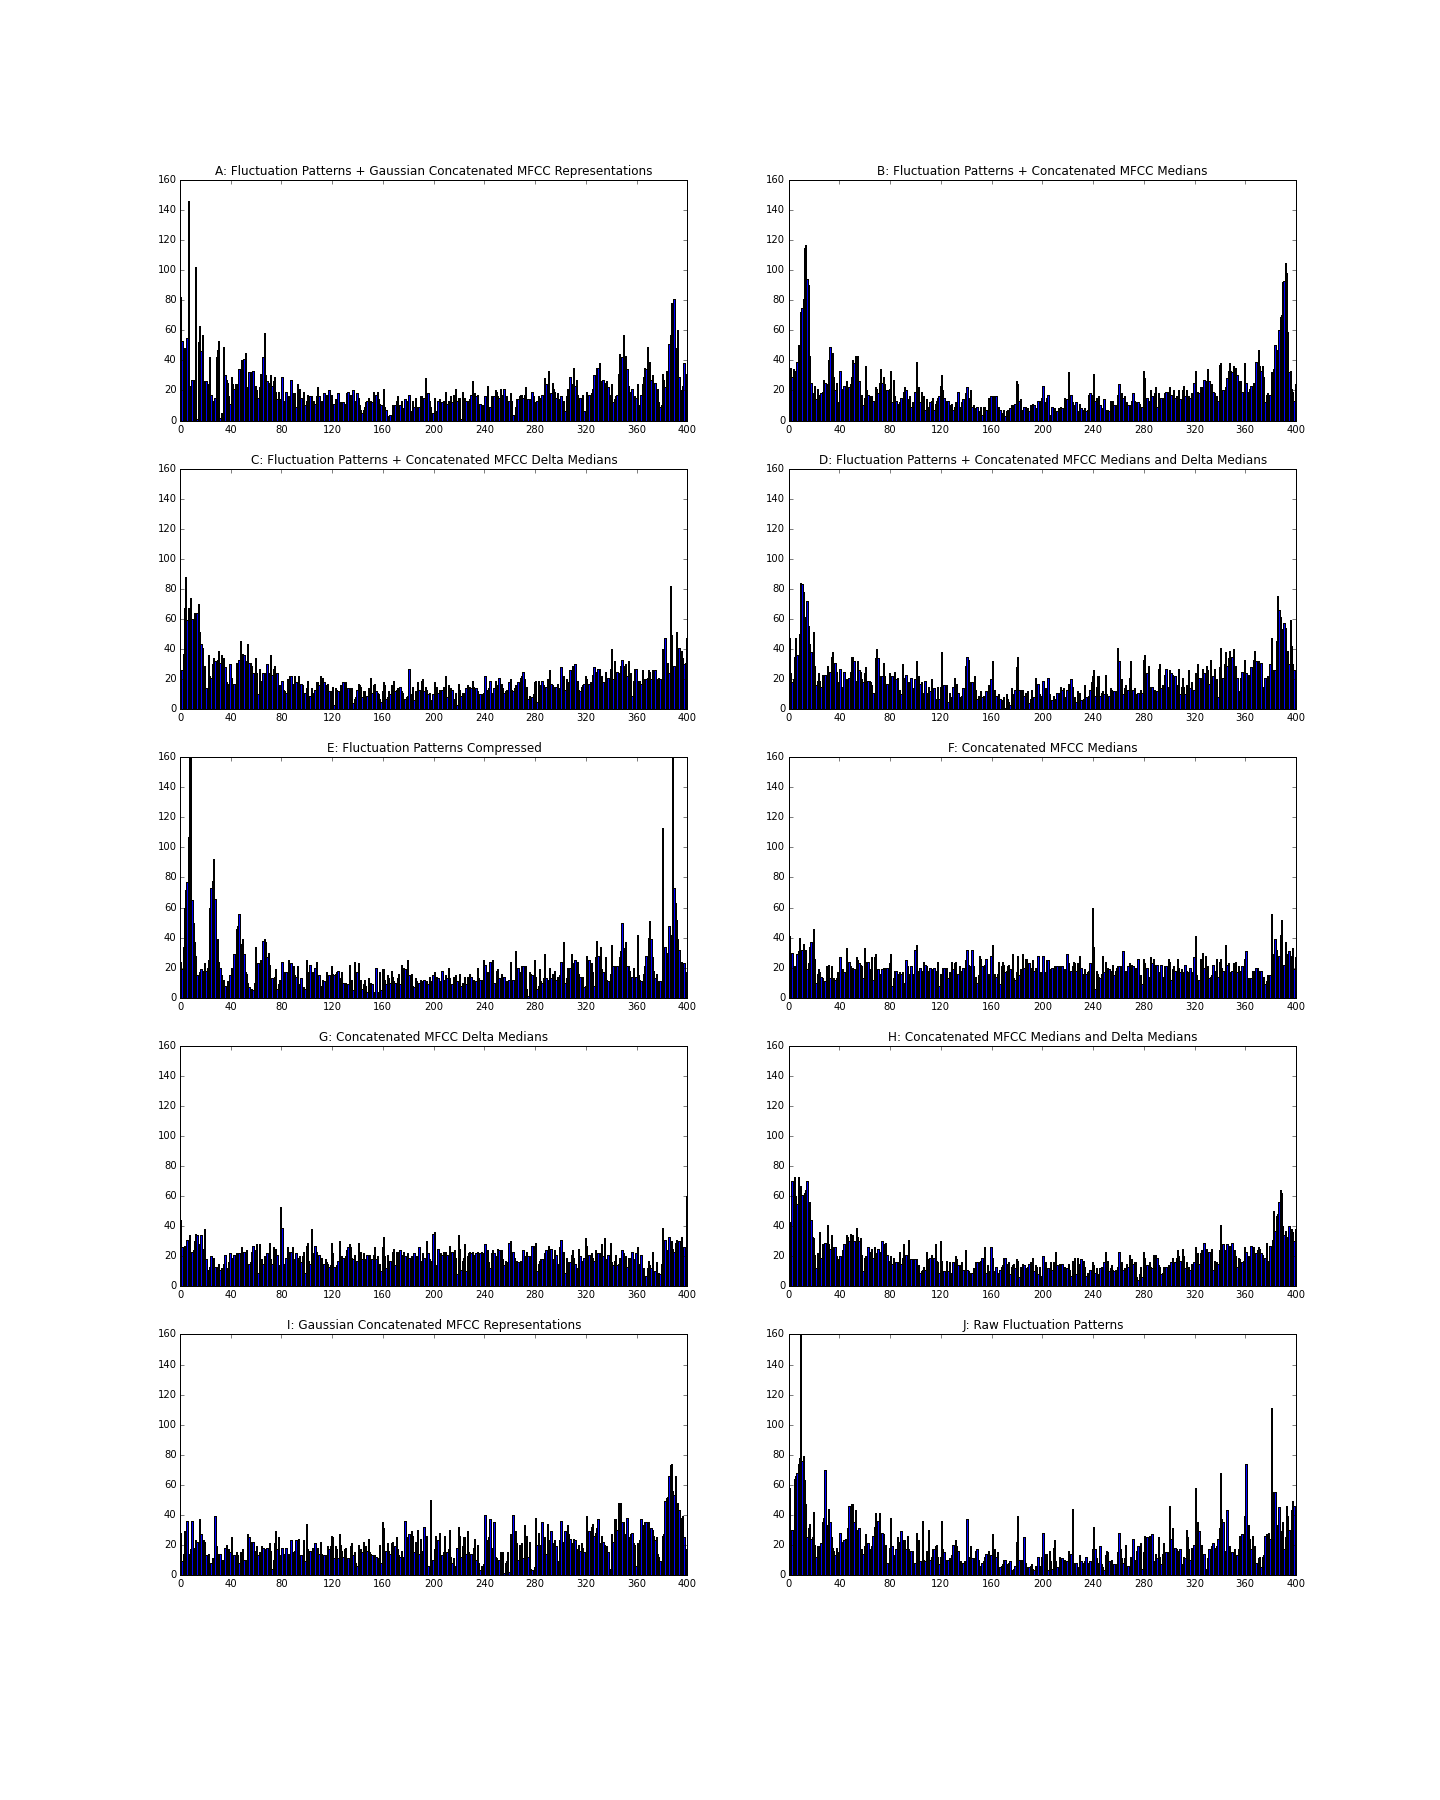
\includegraphics[width=\linewidth]{clusters}
    \end{center}
    \label{fig:clusters}
\end{figure}


\section{Recommender}
To select recommendations for a user the recommender receives a list of tracks the user has liked in the past $L_u$. To do this the recommender does not have to know the track before. If the track is unknown the audio is analysed and the track projected onto a cluster using the SOM algorithm, like presented in the last section. To increase the neighbourhood size we perform a clustering of the codebook with the k-Means algorithm. For each liked tracks the cluster is looked up. Then the clusters are ordered by frequency, in which they in the user's likes. In the following step all tracks from the clusters are retrieved and presented as recommendations after removing the initial likes. Figure \ref{fig:bloc} shows the whole process in a simple diagram. 

\begin{figure}
    \caption{Implemented recommender system}
    \begin{center}
        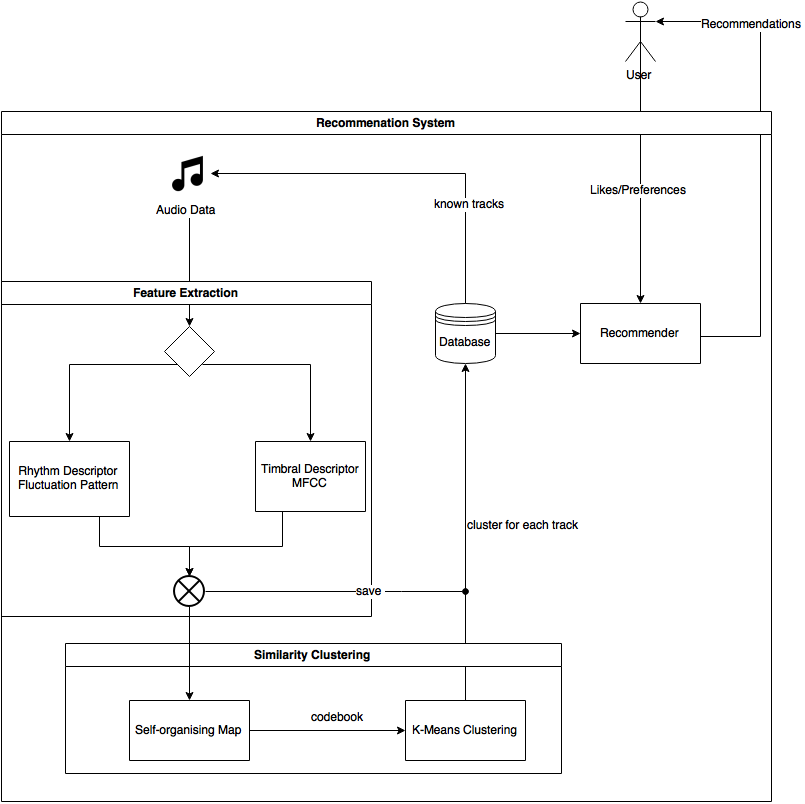
\includegraphics[width=\linewidth]{blockdiag}
    \end{center}
    \label{fig:bloc}
\end{figure}

\subsection{Preferences in Musical Space}
In figure \ref{fig:music_space} we see two different user's preferences mapped onto the k-Means clustered codebook. Each number represents a single like. It can be observed how likes are clearly concentrated in some of the clusters generated by the SOM. Thus we can conclude that similarity might be a valid approach for recommending music. It is also observable that not all likes are in clusters some likes are spread in a random manner over the map, most notably at User 1. This is congruent with humans taste as a lot of people do enjoy bigger variety of styles. Now User 1 has less likes than User 2 so it might be that this user could enjoy music from the clusters he has already likes in. 

\begin{figure}
\centering
\begin{subfigure}{.5\textwidth}
  \centering
  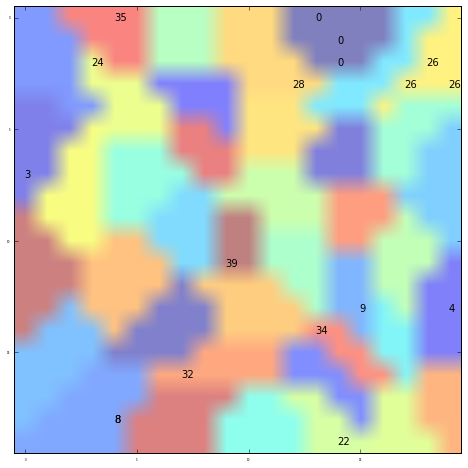
\includegraphics[width=\linewidth]{user1}
  \caption{User 1}
  \label{fig:user1}
\end{subfigure}%
\begin{subfigure}{.5\textwidth}
  \centering
  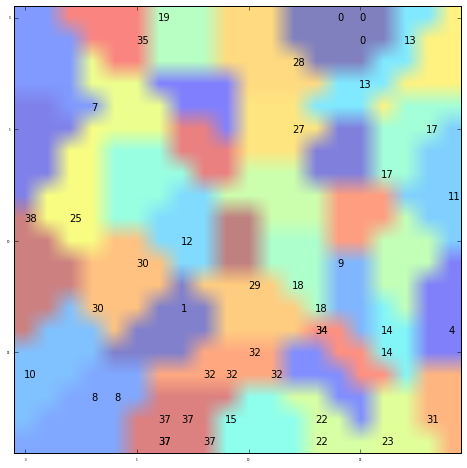
\includegraphics[width=\linewidth]{user2}
  \caption{User 2}
  \label{fig:user2}
\end{subfigure}
\caption{Comparison of two users likes in musical space}
\label{fig:music_space}
\end{figure}


\subsection{Score Calculation}
As one cluster usually holds a big amount of tracks a score is introduced. To calculate the score of a given recommended track $t$ in it's cluster $C_t$ the following formula is used:
\begin{equation}
\begin{split}
s_{u}'(\bm{t}) &=   \min(\bigl\{ \norm{\bm{l_{i}} - \bm{t}} \bigm| l_i \in (C_t \cap L_u) \bigr\}) \\
s_{u}(\bm{t}) &= \frac{1} {s_{u}'(\bm{t})} 
\end{split}
\end{equation}


$s_{u}'(\bm{t})$ presents the minimum distance of the new track to one of the users likes in the track's cluster. This distance is inverted to give a ascending score criterium with decreasing distance. This can be done for each cluster and finally the list of recommendations are sorted using the score criterium. As this step is quite computationally expensive it has been implemented to be optional as selecting tracks from a cluster usually already satisfies a certain proximity to other liked tracks in the cluster. As a solution to this dilemma a whole distance matrix between all tracks of a cluster could be pre-calculated what would reduce computational complexity. Finally the known user likes are removed from the recommended set.


\chapter{Evaluation}
To evaluate the presented algorithm $10\%$ of each user's likes are hidden. Then the different evaluation metrics are calculated for each user. This user scores are averaged and presented in the following tables. Furthermore for reasons of comparison we also evaluate a state of the art CF algorithm \cite{low2014graphlab}. Most tables also include a random recommender to provide a baseline algorithm. This random recommender randomly samples a set of tracks from all available tracks and subtracts the already known user likes.


%To evaluate the feature vectors we used the recall criterium. For each feature vector the clustering  We choose to limit recommendation length by limiting the allowed amount of clusters the algorithm is allowed to use. This results in varying length of recommendations, therefore the table contains in the last column a measure of recommendation length. As can be seen in table \ref{tab:feature_eval} the features vectors B and E perform best. Overall it can be said that the recommendation length has to become quite big to achieve satisfying results. When taking the recommendation length into consideration feature vector B performs the best.


%\subsection{Evaluation by Recall}
%It follows a rather naive evaluation comparing the approach presented here with randomly chosen recommendations as well as with an state of the art collaborative filtering algorithm %(GraphLab). For each user the training set likes are used as input to obtain recommendations. These recommendations are compared to the user's validation set. For each match a true positive was counted. The score is calculated as a percentage of true positives relative to the size of the validation set, also known as recall. As our approach returns quite a lot of clusters for each user, the size of the clusters was limited. To have comparative results with other methods the size of the recommendation lists for all techniques are set to be the same. This recommendation list size depends on the user's training set size. The column recommendation size shows the length of the list relative to all $8003$ tracks. The training set covers about 7400 tracks whereas the complete set consists of 8003, meaning that for about 600 tracks are not known to the CF algorithm, thus they can't be recommended. It should be further mentioned that the CF algorithm calculates a score for each similar item and orders these items based on the calculated score. It considers therefore all items but recommends only the ones with the best score. The CF algorithm never really performs significantly better than the random recommender. This is because due to the fact that the user data is very sparse. 

\subsection{Significance}
We use the sign test to prove that our algorithm performs better than the random recommender. The sign test gives the probability that algorithm A is not truly better than algorithm B. It is counted how often Algorithm A outperforms algorithm B $n_A$ and vice versa $n_B$, while $n=n_A+n_B$. We use as outperform criterium the number of recommended tracks, which appears in the evaluation set. To calculate the significance the formula \ref{form:sign-test} is used. To further evaluate our approach we do the sign test against the random recommender. This test is executed 10 times as the random recommenders performance might vary and the obtained results are averaged. The numbers of cluster to use was set to $40$ and recommendation lists were trimmed afterwards to save computation time. Using this parameters the recommender algorithm's performance should decrease. The obtained probabilities for each feature vector can be observed in Table \ref{tab:sign_test}

\begin{equation} \label{form:sign-test}
p = 0.5^n \sum^n_{i = n_A} \frac{n!}{i!(n-i)!}
\end{equation}

All significance levels below $0.1$ have been printed bold. Usually a algorithm is considered truly better if the sign test evaluates a significance level of $0.05$ or below. It can be seen that only with feature vector H and J a significance level lower than $0.05$ is achieved. As the results for feature vector H are that surprising the experiments have been repeated. This the test was executed 50 times and the results were averaged, resulting in similar probabilities. Also feature vector A achieves sufficient significance but only at very high recommendation lengths. Feature vector D performed quite good on in Table \ref{tab:feature_vec} but never reaches less than $0.09$ significance. 

\begin{table}
\center
\label{tab:sign_test}
\caption{Sign Test probabilities between our approach and random recommender}
\begin{tabular}{| l | c | c | c | c | c | c | c | c | c | c | }
\hline

\rowcolor{lightgray}  N & A & B & C & D & E & F & G & H & I & J  \\ \hline 
$50$		&	$0.83$	&	$0.32$	&	$0.71$	&	$0.64$	&	$0.25$	&	$0.47$	&	$0.57$	&	$\bm{0.07}$	&	$0.75$	&	$0.45$	\\ \hline 
$250$	&	$0.34$	&	$0.44$	&	$0.57$	&	$0.30$	&	$0.15$	&	$0.54$	&	$0.51$	&	$\bm{0.02}$	&	$0.38$	&	$0.31$	\\ \hline 
$1000$	&	$0.41$	&	$0.18$	&	$0.23$	&	$\bm{0.09}$	&	$\bm{0.08}$	&	$0.41$	&	$0.59$	&	$\bm{0.08}$	&	$0.27$	&	$0.13$	\\ \hline 
$2000$	&	$\bm{0.06}$	&	$0.17$	&	$0.22$	&	$0.11$	&	$0.20$	&	$0.47$	&	$0.49$	&	$\bm{0.09}$	&	$0.33$	&	$\bm{0.04}$	\\ \hline 

\end{tabular}
\end{table}
%\begin{table}
%\center
%\caption{Sign Test probabilities between SOM codebook clusters and random recommender}
%\begin{tabular}{| l | r | }
% \hline 
%\rowcolor{lightgray} Recommendation Length & $p$ \\ \hline 
%$5$&$0.5000$\\ \hline
%$20$&$0.8750$\\ \hline
%$100$&$0.0925$\\ \hline
%$500$&$0.1032$\\ \hline
%$1000$&$0.1024$\\ \hline
%$1800$&$\bm{0.0420}$\\ \hline
%\end{tabular}
%\end{table}
\subsection{Feature Vector Evaluation}
To evaluate the feature vectors we used the recall criterium, which is explained later in detail, see \ref{recall}. For now it should be sufficient that it measures how many likes we could predict in relation to all hidden likes. We evaluated different recommendation lengths as well as number of clusters to use over all feature vectors presented in Table \ref{tab:feature_vec}. The recommendation lengths are proportional to the number of clusters used $N_{recommendation} = N_{clusters} * 50$.  Observe as some of them consider rhythm and timbre as for example A and D, while delivering good performance. Others like H, perform quite well but just consider timbre. Others like for example E only consider rhythm and perform very good at lower recommendation lengths but seem to weaken at very high lengths. 

We choose to evaluate further metrics with H as it performed best considering significance levels. Also BAwill be further evaluated as it is a combination of Fluctuation patterns, which reached significance with E and J and the descriptor I which differs in it's representation from the other descriptors. Finally also D will be further considered, as it reached a low significance level and delivered best results in terms of average recall. J will not be further considered as it's use under realistic conditions is difficult because of it's high dimensionality.

\begin{table}
\caption{Feature evaluation table}
\label{tab:feature_eval}
\resizebox{\linewidth}{!}{
\begin{tabular}{| l || c | c | c | c | c |}
 \hline 
\rowcolor{lightgray} & Clusters used & Our Approach & CF Recommender & Random Recommender & Recommendation Size \\ \hline 

\hline \hline \multirow{4}{*}{A} & $1$ &$ 0.87\% (\pm 4.37) $&$ 0.84\% (\pm 4.34) $&$ 0.47\% (\pm 3.62) $&$50$ \\ \cline{2-6} 
& $5$ & $3.86\% (\pm 9.36) $&$ 3.21\% (\pm 8.88) $&$ 3.28\% (\pm 8.93) $&$ 250 $ \\ \cline{2-6} 
& $20$ & $13.89\% (\pm 17.77) $&$ 9.73\% (\pm 13.62) $&$ 12.02\% (\pm 13.96) $&$ 1000 $ \\ \cline{2-6} 
& $40$ & $27.49\% (\pm 21.36) $&$ 18.26\% (\pm 19.34) $&$ 25.40\% (\pm 20.99) $&$ 2000 $ \\ \cline{2-6} 

\hline \hline \multirow{4}{*}{B} & $1$ &$ 0.78\% (\pm 4.23) $&$ 0.84\% (\pm 4.34) $&$ 0.28\% (\pm 1.84) $&$ 50$ \\ \cline{2-6} 
& $5$ & $3.68\% (\pm 8.58) $&$ 3.21\% (\pm 8.88) $&$ 3.58\% (\pm 8.83) $&$ 250 $ \\ \cline{2-6} 
& $20$ & $14.49\% (\pm 18.15) $&$ 9.73\% (\pm 13.62) $&$ 13.19\% (\pm 15.58) $&$ 1000 $ \\ \cline{2-6} 
& $40$ & $26.62\% (\pm 21.08) $&$ 18.26\% (\pm 19.34) $&$ 26.82\% (\pm 21.99) $&$ 2000 $ \\ \cline{2-6} 

\hline \hline \multirow{4}{*}{C} & $1$ &$ 0.62\% (\pm 4.19) $&$ 0.84\% (\pm 4.34) $&$ 0.58\% (\pm 3.40) $&$50$ \\ \cline{2-6} 
& $5$ & $3.72\% (\pm 9.05) $&$ 3.21\% (\pm 8.88) $&$ 2.90\% (\pm 7.79) $&$ 250 $ \\ \cline{2-6} 
& $20$ & $13.12\% (\pm 16.16) $&$ 9.73\% (\pm 13.62) $&$ 12.94\% (\pm 16.34) $&$ 1000 $ \\ \cline{2-6} 
& $40$ & $27.27\% (\pm 21.22) $&$ 18.26\% (\pm 19.34) $&$ 27.75\% (\pm 22.25) $&$ 2000 $ \\ \cline{2-6} 

\hline \hline \multirow{4}{*}{D} & $1$ &$ \bm{1.20\% (\pm 5.82)} $&$ 0.84\% (\pm 4.34) $&$ 0.58\% (\pm 4.12) $&$50$ \\ \cline{2-6} 
& $5$ & $\bm{4.16\% (\pm 11.04)} $&$ 3.21\% (\pm 8.88) $&$ 3.06\% (\pm 7.99) $&$250 $ \\ \cline{2-6} 
& $20$ & $\bm{17.35\% (\pm 19.28)} $&$ 9.73\% (\pm 13.62) $&$ 11.38\% (\pm 15.10) $&$ 1000 $ \\ \cline{2-6} 
& $40$ & $\bm{30.58\% (\pm 23.28)} $&$ 18.26\% (\pm 19.34) $&$ 24.78\% (\pm 21.42) $&$ 2000 $ \\ \cline{2-6} 

\hline \hline \multirow{4}{*}{E} & $1$ &$ 1.12\% (\pm 4.89) $&$ 0.84\% (\pm 4.34) $&$ 0.60\% (\pm 3.11) $&$50$ \\ \cline{2-6} 
& $5$ & $3.80\% (\pm 9.17) $&$ 3.21\% (\pm 8.88) $&$ 2.93\% (\pm 9.00) $&$ 250 $ \\ \cline{2-6} 
& $20$ & $14.36\% (\pm 16.25) $&$ 9.73\% (\pm 13.62) $&$ 12.02\% (\pm 14.59) $&$ 1000 $ \\ \cline{2-6} 
& $40$ & $27.45\% (\pm 21.77) $&$ 18.26\% (\pm 19.34) $&$ 26.85\% (\pm 22.45) $&$ 2000 $ \\ \cline{2-6} 

\hline \hline \multirow{4}{*}{F} & $1$ &$ 0.74\% (\pm 4.17) $&$ 0.84\% (\pm 4.34) $&$ 0.62\% (\pm 3.53) $&$50$ \\ \cline{2-6} 
& $5$ & $3.53\% (\pm 8.82) $&$ 3.21\% (\pm 8.88) $&$ 3.25\% (\pm 9.89) $&$ 250 $ \\ \cline{2-6} 
& $20$ & $13.70\% (\pm 16.81) $&$ 9.73\% (\pm 13.62) $&$ 13.17\% (\pm 17.06) $&$ 1000 $ \\ \cline{2-6} 
& $40$ & $25.46\% (\pm 21.67) $&$ 18.26\% (\pm 19.34) $&$ 25.73\% (\pm 21.97) $&$ 2000 $ \\ \cline{2-6} 

\hline \hline \multirow{4}{*}{G} & $1$ &$ 0.84\% (\pm 4.24) $&$ 0.84\% (\pm 4.34) $&$ 0.73\% (\pm 4.27) $&$50$ \\ \cline{2-6} 
& $5$ & $3.75\% (\pm 9.09) $&$ 3.21\% (\pm 8.88) $&$ 3.22\% (\pm 8.95) $&$ 250 $ \\ \cline{2-6} 
& $20$ & $11.64\% (\pm 15.65) $&$ 9.73\% (\pm 13.62) $&$ 13.27\% (\pm 18.05) $&$ 1000 $ \\ \cline{2-6} 
& $40$ & $25.29\% (\pm 21.48) $&$ 18.26\% (\pm 19.34) $&$ 24.63\% (\pm 21.09) $&$ 2000 $ \\ \cline{2-6} 

\hline \hline \multirow{4}{*}{H} & $1$ &$ 0.86\% (\pm 4.73) $&$ 0.84\% (\pm 4.34) $&$ 1.52\% (\pm 6.75) $&$50$ \\ \cline{2-6} 
& $5$ & $3.61\% (\pm 8.82) $&$ 3.21\% (\pm 8.88) $&$ 2.89\% (\pm 8.17) $&$ 250 $ \\ \cline{2-6} 
& $20$ & $15.23\% (\pm 18.47) $&$ 9.73\% (\pm 13.62) $&$ 11.89\% (\pm 15.13) $&$ 1000 $ \\ \cline{2-6} 
& $40$ & $29.74\% (\pm 22.68) $&$ 18.26\% (\pm 19.34) $&$ 24.77\% (\pm 21.52) $&$ 2000 $ \\ \cline{2-6} 

\hline \hline \multirow{4}{*}{I} & $1$ &$ 0.61\% (\pm 3.58) $&$ 0.84\% (\pm 4.34) $&$ 0.62\% (\pm 3.56) $&$50$ \\ \cline{2-6} 
& $5$ & $3.08\% (\pm 8.79) $&$ 3.21\% (\pm 8.88) $&$ 3.37\% (\pm 9.25) $&$ 250 $ \\ \cline{2-6} 
& $20$ & $13.05\% (\pm 17.11) $&$ 9.73\% (\pm 13.62) $&$ 12.71\% (\pm 16.47) $&$ 1000 $ \\ \cline{2-6} 
& $40$ & $25.07\% (\pm 22.29) $&$ 18.26\% (\pm 19.34) $&$ 25.81\% (\pm 21.06) $&$ 2000 $ \\ \cline{2-6} 

\hline \hline \multirow{4}{*}{J} & $1$ &$ 0.71\% (\pm 4.59) $&$ 0.84\% (\pm 4.34) $&$ 0.57\% (\pm 4.21) $&$50$ \\ \cline{2-6} 
& $5$ & $3.82\% (\pm 9.48) $&$ 3.21\% (\pm 8.88) $&$ 2.92\% (\pm 8.41) $&$ 250 $ \\ \cline{2-6} 
& $20$ & $13.38\% (\pm 16.97) $&$ 9.73\% (\pm 13.62) $&$ 12.39\% (\pm 15.03) $&$ 1000 $ \\ \cline{2-6} 
& $40$ & $26.26\% (\pm 23.12) $&$ 18.26\% (\pm 19.34) $&$ 25.67\% (\pm 21.79) $&$ 2000 $ \\ \cline{2-6}
\end{tabular}	}

\end{table}
%\begin{table}
%\center
%\caption{Sign Test probabilities between k-Means clustered SOM codebook and random recommender}
%\begin{tabular}{| l | r | }
%\hline 
%\rowcolor{lightgray} Recommendation Length & $p$ \\ \hline 
%$5$&$0.5000$\\ \hline
%$20$&$0.8750$\\ \hline
%$100$&$0.9599$\\ \hline
%$500$&$0.4624$\\ \hline
%$1000$&$0.3785$\\ \hline
%$1800$&$\bm{0.0355}$\\ \hline
%\end{tabular}
%\end{table}

\subsection{Measuring Usage Prediction}

As we are using unary ratings the quality of recommendation is measured by introducing metrics of how useful the recommended items are to the user. When evaluating a set of recommendations there are four possible outcomes \ref{tab:outcomes} for the recommended and hidden items.
In offline evaluation we are forced to assume that unused items would have not been used even if the have been recommended. This assumption is in most cases false as a user might use a recommended item and didn't use e.g. like it because he was unaware of it's existence. The following evaluation metrics are proposed by \cite{shani2011evaluating}.

\begin{table}
\center
\caption{Outcomes for unary ratings}
\begin{tabular}{ r | c | c |   }

& Recommended & Not Recommended \\ \hline
Used & True Positive & False Negative   \\ \hline
Not Used & False Positive & True Negative  \\ 

\end{tabular}
\label{tab:outcomes}
\end{table}

\begin{equation}
\text{Precision} = \frac{\vert tp \vert}{\vert tp \vert + \vert fp \vert}
\end{equation}

\begin{equation} \label{recall}
\text{Recall(True Positive Rate)} = \frac{\vert tp \vert}{\vert tp \vert + \vert fn \vert}
\end{equation}

\begin{equation}
\text{False Positive Rate} = \frac{\vert fp \vert}{\vert fp \vert + \vert tn \vert}
\end{equation}

\begin{table}
\center
\caption{Usage Predictions}
\begin{tabular}{| l | c | c | c |}
 \hline 
 \multicolumn{4}{|c|}{Feature Vector A} \\ \hline
\rowcolor{lightgray} $N$ & Precision & Recall & FPR  \\ \hline 

$50$ & $0.104\% (\pm 0.479\%)$& $0.874\% (\pm 4.371\%)$&$ 0.625\% (\pm 0.003\%)$ \\ \hline
$250$ & $0.085\% (\pm 0.178\%)$& $3.865\% (\pm 9.363\%)$&$ 3.123\% (\pm 0.005\%)$ \\ \hline
$1000$ & $0.082\% (\pm 0.105\%)$& $13.888\% (\pm 17.772\%)$&$ 12.494\% (\pm 0.011\%)$ \\ \hline
$2000$ & $0.082\% (\pm 0.078\%)$& $27.492\% (\pm 21.363\%)$&$ 24.988\% (\pm 0.013\%)$ \\ \hline

\multicolumn{4}{|c|}{Feature Vector D} \\ \hline
\rowcolor{lightgray} $N$ & Precision & Recall & FPR  \\ \hline 
$50$ & $0.104\% (\pm 0.479\%)$& $1.204\% (\pm 5.823\%)$&$ 0.625\% (\pm 0.003\%)$ \\ \hline
$250$ & $0.091\% (\pm 0.196\%)$& $4.163\% (\pm 11.044\%)$&$ 3.123\% (\pm 0.006\%)$ \\ \hline
$1000$ & $0.094\% (\pm 0.103\%)$& $17.349\% (\pm 19.277\%)$&$ 12.493\% (\pm 0.011\%)$ \\ \hline
$2000$ & $0.084\% (\pm 0.071\%)$& $30.575\% (\pm 23.279\%)$&$ 24.988\% (\pm 0.014\%)$ \\ \hline

\multicolumn{4}{|c|}{Feature Vector H} \\ \hline
\rowcolor{lightgray} $N$ & Precision & Recall & FPR  \\ \hline 
$50$ & $0.080\% (\pm 0.392\%)$& $0.864\% (\pm 4.729\%)$&$ 0.625\% (\pm 0.002\%)$ \\ \hline
$250$ & $0.078\% (\pm 0.170\%)$& $3.611\% (\pm 8.815\%)$&$ 3.124\% (\pm 0.005\%)$ \\ \hline
$1000$ & $0.086\% (\pm 0.109\%)$& $15.233\% (\pm 18.470\%)$&$ 12.494\% (\pm 0.012\%)$ \\ \hline
$2000$ & $0.085\% (\pm 0.077\%)$& $29.736\% (\pm 22.677\%)$&$ 24.987\% (\pm 0.014\%)$ \\ \hline

\end{tabular}
\label{tab:use}
\end{table}

In Table \ref{tab:use} we see these evaluation metrics on our selected feature vectors. While we can see that descriptor D performs best, the precision is verly low at all times. 
% say something about FPR seems the same for all why?

\subsection{Ranking Measure}
Usually recommendations are presented to a user in an ordered fashion, for example in a horizontal list, with the first element being the most important one. As recommendations lists can be long it is useful to order this list according to the user's preferences. As we have "true" order given for the evaluation set of likes, only the utility of the system's ordering can be measured. The utility of each recommendation is the utility of the recommended item discounted by a factor that depends on its position in the list of recommendations\cite{shani2011evaluating}. The R-Score metric assumes that a user will only see or browse the very first items of a list and the utility of recommended tracks declines exponentially with distance to the first position. Therefore the value of an item only depends on it's position in the recommendation list.

Only with descriptor H we can reach a better result than the random recommender. The random recommender results were averaged over 50 executions of the experiment. The other two descriptor seem to contain most likes very late in the list meaning that the preferences are not as close in space as with descriptor H.

\begin{equation}
R_u = \sum_j \frac{r_{ui_j}}{2^{\frac{j-1}{\alpha - 1}}}
\end{equation}

Where $r_{ui_j} = 1$ if the user $u$ selects item $i$ and $i_j$ is the item at $j^{th}$ position in the list. After obtaining all user's R-Scores the metric can be aggregated using:

\begin{equation}
R =100 \frac{\sum_u R_u}{\sum_u R^*_u}
\end{equation}

with $R^*_u$ being the maximum R-Score that can be obtained by user $u$.

\begin{table}
\center
\caption{RScores}
\begin{tabular}{ r | c | c | c | c | }

\rowcolor{lightgray} Descriptor & A & D & H & Random \\ \hline
R-Score & $0.025$ & $0.052$ & $\bm{0.116}$ & $0.085$   \\

\end{tabular}
\label{tab:rscores}
\end{table}


\subsection{Item Space Coverage}
Item space coverage refers to the proportion of items which can be recommended by the recommender. The item space coverage of our recommender is 100\%. The algorithm is able to recommend each track known to him independently if there is user data available to him. Each track that is in proximity to some like of some user can and will be recommended to this user.

\section{Conclusions}
As seen in evaluation the algorithm presented is yet to improve and to be exposed to different datasets to give a final statement about it's performance. It showed that it has slightly superior performance to the CF algorithm at low recommendations lengths. The significance level is reached by H at a reasonable recommendation length the other feature vectors reach almost significance but only at very high recommendation lengths. Recommendation lists of this size are of low use to the real user. But it also has to be considered that offline evaluation is not an optimal method as it makes some risky assumptions about false positives. It should be also mentioned that on this dataset even the popular collaborative filtering algorithm performed rather poorly not reaching any significance at all even with long recommendation lists. This might be due to the very sparse user data that was given. We had $8003$ tracks and $250$ users. Therefore an matrix with over 2 million entries but only about $14000$ likes were given. That results in a relative population of only $0.7\%$. Also the polyphonic timbre vectors similar as the ones described by \cite{yoshii2008efficient} could not reproduce the results they achieved with they with their model based approach. This might be due to differences in the data used for analysis and evaluation or because concatenated MFCCs are not useful for this method. The data that was used to evaluate their algorithm was not available so the experiments could not be reproduced. It was seen though in \ref{fig:music_space} ,that many user likes form clusters in our music similarity space. Therefore it can be assumed that a certain similarity measure was achieved with this method.

\chapter{Conclusion}

\section{Summary and Discussions}
A recommender system based on audible music similarity was presented. To extract rhythm features Fluctuation Patterns were calculated and to capture musical timbre MFCCs and features based on them were evaluated. This features were used to build an musical space with the SOM algorithm and a recommender was prototyped using this subspace as music similarity measure. We than evaluated the algorithm on a random chosen subset of the Million Song Dataset and compared it to a state of the art CF recommender. Significance over the baseline random recommender could be achieved but mostly at very big recommendation lengths whereas the CF algorithm could not achieve any significance on this data at all. With further adjustments this algorithm could proof useful as a baseline algorithm for systems with sparse user data as it at least performs better than a completely random recommender often used in such situations. The goal has only been reached partially as it could be shown, that likes at least seem to be influenced at least by some similarity measure. Descriptors for music analysis are yet to improve as they usually use methods from speech recognition, which might be not as tailored to the problem as own feature vectors. Also the fluctuation patterns, which were developed especially as music descriptors, have actually shown to be problematic, as some steps do actually worsen the result \cite{lidy2005evaluation}. Subjective listening to single clusters and recommendation has been very interesting and it seems that descriptor D is able span a quite good similarity space as is A. H does certainly introduce a similarity in timbre but subjectively was found to select very dissimilar tracks considering rhythm. Evaluation should be redone on different data to confirm obtained results about significance of this descriptor. 

\section{Reviewing Data and Algorithm}
Below we see a user's like set split into the two sets we used for our evaluation. This split is completely random as no time labels where available for the user data. Therefore this introduces a quite unrealistic model of user's liking data as they are more probable to like data to music they have been listening to more recently. As we see in the picture some tracks are very far away from the main clusters as for example like 11 and 33 are never going to be recommended as they are too far away from all the others and have no neighbour like in their cluster. But the ones in cluster 27 and 36 are likely to be recommended somewhere at bigger recommendation lengths. The highest scores will be given to clusters 19 and 36 as they contain very dense likes so the algorithm will rather recommend likes from this cluster as it assumes that the user has a preference for this kind of music. Considering this information it does make sense why the significance is achieved only at high recommendations lengths.

\begin{figure}
\centering
\begin{subfigure}{.5\textwidth}
  \centering
  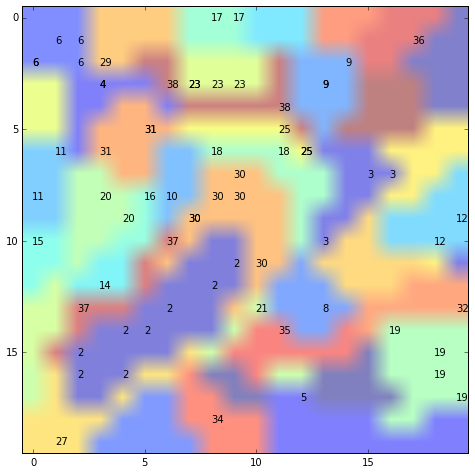
\includegraphics[width=\linewidth]{recs}
  \caption{A subfigure}
  \label{fig:known likes}
\end{subfigure}%
\begin{subfigure}{.5\textwidth}
  \centering
  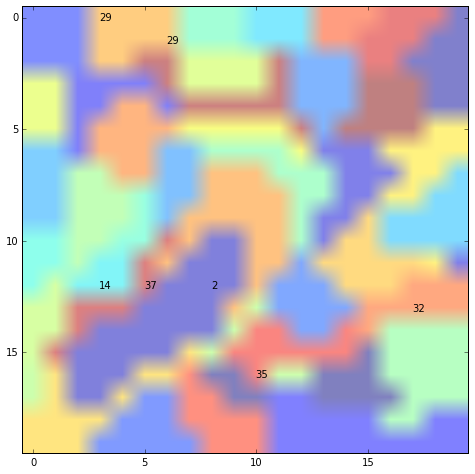
\includegraphics[width=\linewidth]{eval}
  \caption{A subfigure}
  \label{fig:hidden likes}
\end{subfigure}
\caption{The two like sets of a user used for evaluation in music similarity space}
\label{fig:test}
\end{figure}


\section{Future Work}
It stays interesting how this algorithm would perform in an online evaluation which could give concrete insights about how good the calculated musical space is representing actual music similarity even though the concept of similarity might vary drastically between distinct subjects. Then features and clustering algorithm could be adjusted by choosing the best results from online evaluation. For clustering the music space advanced methods like probabilistic methods with soft cluster or hierarchical techniques, which subdivide big clusters further, could be used to cluster this rather complex space. Furthermore it would be interesting to construct a system that learns similarity from a users listening history, so it adjust it's similarity measure to the individual.

\bibliographystyle{abntex2-alf}
\bibliography{biblio}

\end{document}
